% ******************************* PhD Thesis Template **************************
% Please have a look at the README.md file for info on how to use the template

\documentclass[a4paper,oneside,12pt,times,numbered,print,index,custombib]{PhDThesisPSnPDF}

\usepackage[english,italian]{babel}

% ******************************************************************************
% ******************************* Class Options ********************************
% *********************** See README for more details **************************
% ******************************************************************************

% `a4paper'(The University of Cambridge PhD thesis guidelines recommends a page
% size a4 - default option) or `a5paper': A5 Paper size is also allowed as per
% the Cambridge University Engineering Deparment guidelines for PhD thesis
%
% `11pt' or `12pt'(default): Font Size 10pt is NOT recommended by the University
% guidelines
%
% `oneside' or `twoside'(default): Printing double side (twoside) or single
% side.
%
% `print': Use `print' for print version with appropriate margins and page
% layout. Leaving the options field blank will activate Online version.
%
% `index': For index at the end of the thesis
%
% `draftclassic': For draft mode without loading any images (same as draft in book)
%
% `draft': Special draft mode with line numbers, images, and water mark with
% timestamp and custom text. Position of the text can also be modified.
%
% `abstract': To generate only the title page and abstract page with
% dissertation title and name, to submit to the Student Registry
%
% `chapter`: This option enables only the specified chapter and it's references
%  Useful for review and corrections.
%
% ************************* Custom Page Margins ********************************
%
% `custommargin`: Use `custommargin' in options to activate custom page margins,
% which can be defined in the preamble.tex. Custom margin will override
% print/online margin setup.
%
% *********************** Choosing the Fonts in Class Options ******************
%
% `times' : Times font with math support. (The Cambridge University guidelines
% recommend using times)
%
% `fourier': Utopia Font with Fourier Math font (Font has to be installed)
%            It's a free font.
%
% `customfont': Use `customfont' option in the document class and load the
% package in the preamble.tex
%
% default or leave empty: `Latin Modern' font will be loaded.
%
% ********************** Choosing the Bibliography style ***********************
%
% `authoryear': For author-year citation eg., Krishna (2013)
%
% `numbered': (Default Option) For numbered and sorted citation e.g., [1,5,2]
%
% `custombib': Define your own bibliography style in the `preamble.tex' file.
%              `\RequirePackage[square, sort, numbers, authoryear]{natbib}'.
%              This can be also used to load biblatex instead of natbib
%              (See Preamble)
%
% **************************** Choosing the Page Style *************************
%
% `default (leave empty)': For Page Numbers in Header (Left Even, Right Odd) and
% Chapter Name in Header (Right Even) and Section Name (Left Odd). Blank Footer.
%
% `PageStyleI': Chapter Name next & Page Number on Even Side (Left Even).
% Section Name & Page Number in Header on Odd Side (Right Odd). Footer is empty.
%
% `PageStyleII': Chapter Name on Even Side (Left Even) in Header. Section Number
% and Section Name in Header on Odd Side (Right Odd). Page numbering in footer

% Uncomment to change page style
\pagestyle{PageStyleII}


% ********************************CUSTOM SETTINGS ********************************
\usepackage{amsmath}
\usepackage{graphicx}
\usepackage[table,xcdraw]{xcolor}
\usepackage[colorinlistoftodos]{todonotes}
\usepackage{url}
\usepackage{subcaption} 
\usepackage{wrapfig}
\usepackage{listings}
\usepackage{epigraph}
%\usepackage[dvipsnames]{xcolor}
%\usepackage{wrapfig}
%\usepackage{graphicx}
\usepackage[table,xcdraw]{xcolor}
\usepackage{color}


%%%%%%%%%%%%%%%%%%%%%%%% per immagini e tabelle di fianco %%%%%%%%%%%%%%%%%%%%%%%% 
%%%%%%%%%%%% https://tex.stackexchange.com/questions/265889/table-and-figure-side-by-side-with-minipages
\usepackage{booktabs}
\usepackage{varwidth}

%%%%%%%%%%%%%%%%% per grafici e tabelle insieme
%%%%%%%%%%%% https://tex.stackexchange.com/questions/6850/table-and-figure-side-by-side-with-independent-captions
\usepackage{floatrow}
% Table float box with bottom caption, box width adjusted to content
\newfloatcommand{capbtabbox}{table}[][\FBwidth]

%%%%%%%%%%%%%%%%% per le citazioni
\usepackage{microtype}



%%% aggiunto da https://github.com/lucach/frontespizio-unimib/


\usepackage{hyperref}
\usepackage[T1]{fontenc}
\usepackage[utf8]{inputenc}
\usepackage{setspace}
%\usepackage[paper=a4paper,margin=1in]{geometry}



%New colors defined below
\definecolor{codegreen}{rgb}{0,0.6,0}
\definecolor{codegray}{rgb}{0.5,0.5,0.5}
\definecolor{codepurple}{rgb}{0.58,0,0.82}
\definecolor{backcolour}{rgb}{0.95,0.95,0.92}

%Code listing style named "mystyle"
\lstdefinestyle{mystyle}{
  backgroundcolor=\color{backcolour},   commentstyle=\color{codegreen},
  keywordstyle=\color{magenta},
  numberstyle=\tiny\color{codegray},
  stringstyle=\color{codepurple},
  basicstyle=\footnotesize,
  breakatwhitespace=false,         
  breaklines=true,                 
  captionpos=b,                    
  keepspaces=true,                 
  numbers=left,                    
  numbersep=5pt,                  
  showspaces=false,                
  showstringspaces=false,
  showtabs=false,                  
  tabsize=2
}
%"mystyle" code listing set
\lstset{style=mystyle}

%\usepackage[savemem]{listings}
\linespread{1.5}

\usepackage[linesnumbered,vlined,ruled,italiano]{algorithm2e}
\usepackage{amssymb}
\usepackage{minted}
\usepackage{rotating}
\usepackage{lscape}

\renewcommand{\listingscaption}{Listato}

\renewcommand{\listoflistingscaption}{Elenco dei listati}




%\usepackage{listings}




\usepackage[nolist]{acronym} %http://ctan.org/pkg/acronym



% ********************************** Preamble **********************************
% Preamble: Contains packages and user-defined commands and settings
% ******************************************************************************
% ****************************** Custom Margin *********************************

% Add `custommargin' in the document class options to use this section
% Set {innerside margin / outerside margin / topmargin / bottom margin}  and
% other page dimensions
\ifsetCustomMargin
  \RequirePackage[left=30mm,right=30mm,top=35mm,bottom=30mm,footnotesep=3cm]{geometry}
  \setFancyHdr % To apply fancy header after geometry package is loaded
\fi

% Add spaces between paragraphs
%\setlength{\parskip}{0.5em}
% Ragged bottom avoids extra whitespaces between paragraphs
\raggedbottom
% To remove the excess top spacing for enumeration, list and description
\usepackage{enumitem}
\setlist[enumerate,itemize,description]{topsep=0em}
% remove space between list items
\setlist[itemize]{nolistsep}
\setlist[enumerate]{nolistsep}


% *****************************************************************************
% ******************* Fonts (like different typewriter fonts etc.)*************

% Add `customfont' in the document class option to use this section

\ifsetCustomFont
  % Set your custom font here and use `customfont' in options. Leave empty to
  % load computer modern font (default LaTeX font).
  %\RequirePackage{helvet}

  % For use with XeLaTeX
  %  \setmainfont[
  %    Path              = ./libertine/opentype/,
  %    Extension         = .otf,
  %    UprightFont = LinLibertine_R,
  %    BoldFont = LinLibertine_RZ, % Linux Libertine O Regular Semibold
  %    ItalicFont = LinLibertine_RI,
  %    BoldItalicFont = LinLibertine_RZI, % Linux Libertine O Regular Semibold Italic
  %  ]
  %  {libertine}
  %  % load font from system font
  %  \newfontfamily\libertinesystemfont{Linux Libertine O}
\fi

% *****************************************************************************
% **************************** Custom Packages ********************************

% ************************* Algorithms and Pseudocode **************************

%\usepackage{algpseudocode}


% ********************Captions and Hyperreferencing / URL **********************

% Captions: This makes captions of figures use a boldfaced small font.
%\RequirePackage[small,bf]{caption}

\RequirePackage[labelsep=space,tableposition=top]{caption}
\renewcommand{\figurename}{Fig.} %to support older versions of captions.sty


% *************************** Graphics and figures *****************************

%\usepackage{rotating}
%\usepackage{wrapfig}

% Uncomment the following two lines to force Latex to place the figure.
% Use [H] when including graphics. Note 'H' instead of 'h'
%\usepackage{float}
%\restylefloat{figure}

% Subcaption package is also available in the sty folder you can use that by
% uncommenting the following line
% This is for people stuck with older versions of texlive
%\usepackage{sty/caption/subcaption}

% \usepackage{subcaption}
\usepackage[font={footnotesize, it}]{caption}


% ********************************** Tables ************************************
\usepackage{booktabs} % For professional looking tables
\usepackage{multirow}

%\usepackage{multicol}
%\usepackage{longtable}
%\usepackage{tabularx}


% *********************************** SI Units *********************************
\usepackage{siunitx} % use this package module for SI units


% ******************************* Line Spacing *********************************

% Choose linespacing as appropriate. Default is one-half line spacing as per the
% University guidelines

% \doublespacing
% \onehalfspacing
% \singlespacing


% ************************ Formatting / Footnote *******************************

% Don't break enumeration (etc.) across pages in an ugly manner (default 10000)
%\clubpenalty=500
%\widowpenalty=500

%\usepackage[perpage]{footmisc} %Range of footnote options

% increase space between text and footnotes
\setlength{\skip\footins}{8mm}

% *****************************************************************************
% *************************** Bibliography  and References ********************

%\usepackage{cleveref} %Referencing without need to explicitly state fig /table

% Add `custombib' in the document class option to use this section
%\ifuseCustomBib
%   \RequirePackage[square, sort, numbers, authoryear]{natbib} % CustomBib

% If you would like to use biblatex for your reference management, as opposed to the default `natbibpackage` pass the option `custombib` in the document class. Comment out the previous line to make sure you don't load the natbib package. Uncomment the following lines and specify the location of references.bib file

\RequirePackage[backend=biber, style=numeric-comp, citestyle=numeric, sorting=nty]{biblatex}
\addbibresource{references/references.bib} %Location of references.bib only for biblatex, Do not omit the .bib extension from the filename.

%\fi

% changes the default name `Bibliography` -> `References'
\renewcommand{\bibname}{References}


% ******************************************************************************
% ************************* User Defined Commands ******************************
% ******************************************************************************

% *********** To change the name of Table of Contents / LOF and LOT ************

%\renewcommand{\contentsname}{My Table of Contents}
%\renewcommand{\listfigurename}{My List of Figures}
%\renewcommand{\listtablename}{My List of Tables}


% ********************** TOC depth and numbering depth *************************

\setcounter{secnumdepth}{2}
\setcounter{tocdepth}{2}


% ******************************* Nomenclature *********************************

% To change the name of the Nomenclature section, uncomment the following line

\renewcommand{\nomname}{Nomenclatura}


% ********************************* Appendix ***********************************

% The default value of both \appendixtocname and \appendixpagename is `Appendices'. These names can all be changed via:

%\renewcommand{\appendixtocname}{List of appendices}
%\renewcommand{\appendixname}{Appndx}

% *********************** Configure Draft Mode **********************************

% Uncomment to disable figures in `draft'
%\setkeys{Gin}{draft=true}  % set draft to false to enable figures in `draft'

% These options are active only during the draft mode
% Default text is "Draft"
%\SetDraftText{DRAFT}

% Default Watermark location is top. Location (top/bottom)
%\SetDraftWMPosition{bottom}

% Draft Version - default is v1.0
%\SetDraftVersion{v1.1}

% Draft Text grayscale value (should be between 0-black and 1-white)
% Default value is 0.75
%\SetDraftGrayScale{0.8}


% ******************************** Todo Notes **********************************
%% Uncomment the following lines to have todonotes.

%\ifsetDraft
%	\usepackage[colorinlistoftodos]{todonotes}
%	\newcommand{\mynote}[1]{\todo[author=kks32,size=\small,inline,color=green!40]{#1}}
%\else
%	\newcommand{\mynote}[1]{}
%	\newcommand{\listoftodos}{}
%\fi

% Example todo: \mynote{Hey! I have a note}

% *****************************************************************************
% ******************* Better enumeration my MB*************
\usepackage{enumitem}



% ************************ Thesis Information & Meta-data **********************
% Thesis title and author information, refernce file for biblatex
% ************************ Thesis Information & Meta-data **********************
%% The title of the thesis
\title{}
%\texorpdfstring is used for PDF metadata. Usage:
%\texorpdfstring{LaTeX_Version}{PDF Version (non-latex)} eg.,
%\texorpdfstring{$sigma$}{sigma}

%% Subtitle (Optional)
\subtitle{Using the CUED template}

%% The full name of the author
\author{Krishna Kumar}

%% Department (eg. Department of Engineering, Maths, Physics)
\dept{Department of Engineering}

%% University and Crest
\university{University of Cambridge}
% Crest minimum should be 30mm.
\crest{\includegraphics[width=0.2\textwidth]{University_Crest}}
%% Use this crest, if you are using the college crest
%% Crest long miminum should be 65mm
%\crest{\includegraphics[width=0.45\textwidth]{University_Crest_Long}}

%% College shield [optional] 
% Crest minimum should be 30mm.
%\collegeshield{\includegraphics[width=0.2\textwidth]{CollegeShields/Kings}}


%% Supervisor (optional)
%% for multiple supervisors, append each supervisor with the \newline command
%\supervisor{Prof. A.B. Supervisor\newline
%Prof. C.D. Supervisor}

%% Supervisor Role (optional) - Supervisor (default) or advisor
% \supervisorrole{\textbf{Supervisors: }}
%% if no title is desired:
% \supervisorrole{}

%% Supervisor line width: required to align supervisors
%\supervisorlinewidth{0.35\textwidth}

%% Advisor (optional)
%% for multiple advisors, append each advisor with the \newline command
%\advisor{Dr. A. Advisor\newline
%Dr. B. Advisor}
     
%% Advisor Role (optional) - Advisor (default) or leave empty
% \advisorrole{Advisors: }
%% if no title is required
% \advisorrole{}

%% Advisor line width: required to align supervisors
%\advisorlinewidth{0.25\textwidth}


%% You can redefine the submission text:
% Default as per the University guidelines:
% ``This dissertation is submitted for the degree of''
%\renewcommand{\submissiontext}{change the default text here if needed}

%% Full title of the Degree
\degreetitle{Tesi Triennale - Informatica }

%% College affiliation (optional)
\college{Università degli Studi di Milano - Bicocca}

%% Submission date
% Default is set as {\monthname[\the\month]\space\the\year}
%\degreedate{September 2014} 

%% Meta information
\subject{LaTeX} \keywords{{LaTeX} {PhD Thesis} {Engineering} {University of
Cambridge}}


% ***************************** Abstract Separate ******************************
% To printout only the titlepage and the abstract with the PhD title and the
% author name for submission to the Student Registry, use the `abstract' option in
% the document class.

\ifdefineAbstract
 \pagestyle{empty}
 \includeonly{Declaration/declaration, abstract}
\fi

% ***************************** Chapter Mode ***********************************
% The chapter mode allows user to only print particular chapters with references
% Title, Contents, Frontmatter are disabled by default
% Useful option to review a particular chapter or to send it to supervisior.
% To use choose `chapter' option in the document class

\ifdefineChapter
 \includeonly{chapter3}
\fi


% ********************************CUSTOM TITLE STYLE ********************************
\usepackage{titlesec}
\newcommand{\chapnumfont}{%     % define font for chapter number
  \usefont{T1}{pnc}{b}{n}%      % choose New Chancery, bold, normal shape
  \fontsize{100}{100}%          % font size 100pt, baselineskip 100pt
  \selectfont%                  % activate font
}
\colorlet{chapnumcol}{gray!75}
\titleformat{\chapter}[display]
{\filleft\bfseries}
{\filleft\chapnumfont\textcolor{chapnumcol}{\thechapter}}
{-24pt}
{\Huge}





% ******************************** Front Matter ********************************
\begin{document}

\frontmatter

%\maketitle


\begin{titlepage}
    
    \noindent
    \begin{minipage}[t]{0.19\textwidth}
        \vspace{-4mm}{
\includegraphics[scale=1.15]{pics/logo_unimib.pdf}}
    \end{minipage}
    \begin{minipage}[t]{0.81\textwidth}
    {
            \setstretch{1.42}
            {\textsc{Università degli Studi di Milano - Bicocca}} \\
            \textbf{Scuola di Scienze} \\
            \textbf{Dipartimento di Informatica, Sistemistica e Comunicazione} \\
            \textbf{Corso di laurea in Informatica} \\
            \par
    }
    \end{minipage}
    
\vspace{40mm}
    
\begin{center}
        {\LARGE{
                \setstretch{1.2}
                \textbf{Tecniche di Natural Language Processing \\ per il riconoscimento dei discorsi d'odio sui social network}
                \par
        }}
    \end{center}
    
    % default 50mm:
    %\vspace{50mm}
    \vspace{25mm}
    
    \noindent
    {\large \textbf{Relatore:} Prof.ssa Elisabetta Fersini} \\

    \noindent
    {\large \textbf{Correlatore:} Prof. Antonio Candelieri}
    
    \vspace{15mm}

    \begin{flushright}
        {\large \textbf{Relazione della prova finale di:}} \\
        \large{Daniel Scalena} \\
        \large{Matricola 844608} 
    \end{flushright}
    
    % default 40mm:
    %\vspace{40mm}
    \vspace{20mm}
    
    \begin{center}
        {\large{\bf Anno Accademico 2020-2021}}
    \end{center}

    \restoregeometry
    
\end{titlepage}



%\include{Dedication/dedication}
%\include{Declaration/declaration}

\include{Abstract/abstract}

% *********************** Adding TOC and List of Figures ***********************


\tableofcontents
%\listoffigures


% \printnomenclature[space] space can be set as 2em between symbol and description
%\printnomenclature[3em]

\printnomenclature

% ******************************** Main Matter *********************************

\mainmatter


%!TEX root = ../thesis.tex
%*******************************************************************************
%****************************** Third Chapter **********************************
%*******************************************************************************
\chapter{Introduzione}
\hspace{0,5cm} 
\section{Il problema dei contenuti offensivi nei social Network}

L'uso dei social network è ormai da molti anni entrato nelle abitudini quotidiane di una gran parte della popolazione mondiale: il loro uso semplice e immediato permette a persone di ogni età di interfacciarsi con un mondo infinito di informazioni che rispecchiano la realtà che ordinariamente ci circonda. Tra le innumerevoli opportunità offerte e gli enormi vantaggi della vita online spesso la regolarizzazione dei contenuti non riesce a mantenere il passo. Risolvere questo problema rappresenta un'ardua sfida sopratutto in un mondo virtuale dove la possibilità di mantenere una pseudo anonimità rende il lavoro di gran lunga più complicato che nel mondo reale.

La quantità di dati presenti sulle piattaforme social supera di gran lunga la capacità di controllo a disposizione delle aziende proprietarie e per questo motivo, solamente negli ultimi anni, la ricerca si sta orientando verso il riconoscimento automatico dei contenuti offensivi. Il compito di supervisionare e riconoscere violazioni delle norme di servizio, o in questo caso quello che è in gergo chiamato \textit{hate speech}, è tuttora affidato a un gruppo ristretto di lavoratori chiamati ironicamente "\textit{Deciders}" \cite{Deciders}. Nonostante gli aiuti forniti da algoritmi di riconoscimento automatico, rimane comunque necessaria una supervisione umana che implica un lavoro decisamente più grande di quello che si possa comunemente immaginare. Il perfezionamento di algoritmi in grado di riconoscere automaticamente contenuti offensivi risulta quindi essere sempre più una questione di urgenza e di assoluta priorità per tutelare nel miglior modo possibile gli utenti che frequentano quotidianamente le piattaforme social.



\subsection{Panoramica generale su TikTok}
    Tra tutti i diversi social network, ormai consolidati e conosciuti da diversi anni, TikTok risulta essere non solo l'ultimo arrivato ma anche quello che sta subendo una crescita maggiore nell'ultimo periodo. Il suo ambiente, frequentato prevalentemente da giovanissimi, lo rende per sua stessa natura in continua evoluzione con trand che ne cambiano le modalità di utilizzo quasi giornalmente. Allo stato attuale il controllo dei contenuti offensivi è eseguito principalmente in maniera manuale basandosi sulla sola segnalazione degli utenti o sull'azione dei moderatori che creano i contenuti sulla piattaforma.
    La mancanza di un sistema automatico efficace in grado di classificare ciò che risulta essere offensivo rende complicato contenere, sopratutto in caso di creator con un grande seguito, i discorsi d'odio sulla piattaforma.

    L'obiettivo è quindi migliorare gli strumenti di identificazione fornendosi delle più recenti ricerche nel campo del riconoscimento del linguaggio naturale per rendere TikTok, o più in generale ogni piattaforma social online, un luogo virtuale più sicuro per le persone che lo frequentano ogni giorno.

\section{Presentazione del lavoro svolto}

La ricerca di un sistema di classificazione efficace, capace di comprendere le più piccole sfumature del linguaggio sapendone interpretare ogni piccolo aspetto, è sempre stato tra i compiti più difficili per dei sistemi automatici privi di esperienza. Il lavoro svolto mira a fornire una soluzione efficace a questo problema esplorando le varie possibilità offerte della comunità scientifica nel campo del riconoscimento del linguaggio naturale e, in particolare, vengono proposte diverse soluzioni in grado di identificare i discorsi d'odio. 

Come primo approccio è stato progettato un sistema capace di riconoscere parole offensive e denigratorie nei commenti scaricati: i risultati ottenuti non riescono ad essere sufficientemente precisi nell'identificazione dei commenti negativi, problematica dovuta ad una serie di caratteristiche legate alla comunicazione su TikTok. 
Una valida alternativa è rappresentata dall'utilizzo di reti neurali profonde in grado di apprendere al meglio il contesto di un commento. Attualmente lo stato dell'arte è rappresentato dai modelli BERT di Google la cui capacità di codifica del testo riesce efficacemente nella rappresentazione di ogni parola nel contesto entro la quale è inserita. I risultati di questo approccio risultano essere più che validi se confrontati con gli stessi ottenuti dalla classificazione lessicale. 
Viene infine proposto un ultimo lavoro di ottimizzazione, modificando la rete neurale originale e cercando di migliorarne le relative le prestazioni. Il sistema risultante evidenzia un'ottima performance tanto da riuscire nella maggior parte dei casi a comprendere appieno il contesto e il senso dei commenti pubblicati online.
%!TEX root = ../thesis.tex
%*******************************************************************************
%****************************** Third Chapter **********************************
%*******************************************************************************
\chapter{Stato dell'arte}
\hspace{0,5cm}

\section{Definizione dei discorsi d'odio}
Nonostante la grande presenza di discorsi d'odio nel panorama dei social network, non è ancora presente una definizione nitida e universale che riesca a inquadrare il fenomeno entro una cornice precisa. Le diverse definizioni, di quello che è comunemente chiamato \textit{hate speech}, sono principalmente fornite da organizzazioni sovranazionali come l'Unione Europea in \cite{hatespeechEU}, da organizzazioni internazionali per le minoranze (ILGA \cite{ilga}), da documenti scientifici e dai termini e condizioni delle principali compagnie tecnologiche operanti nel settore social (Facebook, YouTube e Twitter in \cite{facebookhate,youtubehate,twitterhate}).

In \cite{survey2} viene svolto un lavoro di analisi su queste fonti e vengono sommarizzate efficacemente fornendo la seguente definizione tradotta di \textit{hate speech}:

\begin{quote}
    \textit{Il discorso d'odio è un linguaggio che attacca o sminuisce, incita violenza o odio verso dei gruppi, basandosi su specifiche caratteristiche quali l'apparenza fisica, la religione, la discendenza, la nazionalità o le origini etniche, l'orientamento sessuale, l'identità di genere o altro, e può verificarsi in diversi stili linguistici, anche in forma subdola o con l'uso di umorismo.}
\end{quote}

Su questa definizione appena introdotta si baserà il lavoro svolto per la classificazione dei contenuti d'odio online.



\section{Lavori relativi al riconoscimento dei discorsi d'odio}

Il problema di riconoscimento dei discorsi d'odio sui social network, seppur sia ancora nella sua fase iniziale, è in rapida evoluzione. Ad esempio, non è ancora presente un benchmark universale per testare le performance di una qualsiasi tecnica utilizzata e la gran parte dei testi usati per la classificazione vengono generati caso per caso, variando di molto il tipo di linguaggio utilizzato \cite{hatespeechSurvey}, tuttavia è presente un vasto numero di metodologie in grado di identificare testi offensivi e denigratori. Eccezion fatta per pochi casi (\cite{fersES,HateData1,HateData2,HateData3,HateData4}), la stragrande maggioranza di dataset rimangono spesso privati, limitando la possibilità di eventuali confronti tra diversi metodi di classificazione.
Un’ulteriore problematica presente nel settore è costituita dalla scarsa variabilità relativa ai social network utilizzati, difatti la maggior parte degli studi usa Twitter come unica piattaforma per la raccolta di informazioni. Tra le probabili cause di questo fenomeno è sicuramente presente l'oggettiva difficoltà riscontrata durante la raccolta dei dati, molte volte limitata o perfino bloccata dalle stesse piattaforme social per tutelare la privacy dei propri utenti. Esplorando la letteratura presente è inoltre evidente come la lingua più analizzata sia l’inglese, con alcune più rare eccezioni per le lingue europee più diffuse quali tedesco, spagnolo, francese e italiano, rimanendo comunque poco sufficienti a fornire un quadro chiaro della situazione dei fenomeni di odio online nei diversi paesi del mondo.

Diversi studi sono stati effettuati con lo scopo di riconoscere i diversi tipi di hate speech online classificandoli in base ai loro attributi: nella maggior parte dei casi le statistiche descrittive evidenziano una forte presenza di razzismo \cite{LocateHate}, sessismo e misoginia \cite{SarahMiso,fersES,JamieMiso}, pregiudizi contro immigrati \cite{rnnabusive} e omofobia \cite{VasuHomophobia}. Nonostante la presenza di diverse categorie però, una gran parte degli studi si concentra su una classificazione esclusivamente binaria, lasciando in sospeso ad eventuali sviluppi futuri il riconoscimento di tutte le sottocategorie precedentemente elencate.


Il riconoscimento dei discorsi d’odio online viene svolto attraverso tecniche di text mining, ovvero un'analisi del lessico utilizzato nei dati relativi alla ricerca. Generalmente vengono prese in considerazione diverse caratteristiche dei testi per trovare la/e combinazioni che permettono una migliore classificazione dei discorsi d’odio.


\subsection{Dizionari}

La strategia più semplice utilizzata per l’analisi dei testi è sicuramente l’uso dei dizionari, ossia raccolte di parole offensive e denigratorie che vengono generalmente usate in commenti contenenti discorsi d’odio. Contando il numero di occorrenze delle parole offensive o usando la normalizzazione sulla base della lunghezza del testo considerato, è possibile generare un punteggio che indichi con quanta probabilità il commento appartenga alla classe dei discorsi d’odio.

Diversi miglioramenti a questo approccio vengono evidenziati in studi \cite{WilliamHate, languagedetect,SriCyberbullying} che fanno uso della \textit{distance metric}, una tecnica in grado di mitigare il problema del mascheramento delle parole. Questa procedura, usata dagli utenti online per ingannare il riconoscimento automatico dei termini offensivi, riguarda nella maggior parte dei casi la sostituzione di un carattere all’interno di una parola pur mantenendone un aspetto visivo simile all’originale. Come esempio esplicativo, calcolando il minimo numero di modifiche da apportare la parola mascherata “\textit{stup1d0}”, è possibile associarla alla sua forma originale “\textit{stupido}”, presente in un qualsiasi dizionario come termine chiaramente offensivo.

Il confronto tra i testi esaminati e i dizionari contenenti parole offensive come \cite{Hurtlex,ShuhuaDict,KarthikDict,MaralDict} riesce nella maggior parte dei casi a individuare i commenti negativi, pur mancando ancora di precisione nella divisione delle classi e generando una grande quantità di falsi positivi. Osservando il lavoro svolto in \cite{cyberbullying} è evidente come una classificazione di questo tipo sia inefficace nel rappresentare il contesto entro il quale un determinato termine è inserito: secondo lo studio il 48\% dei testi presi in esame non rientra nella classe dei negativi nonostante contenga un’alta percentuale di parole denigratorie.

Un ulteriore supporto per la classificazione viene fornito dall'analisi di diversi fattori concorrenti ad un probabile atteggiamento denigratorio da parte di un commento \cite{Chen,offensivelang}. Osservando i riferimenti esterni come URL o hashtag è generalmente possibile attribuire un contesto entro il quale il testo in analisi è inserito o, analizzando la sua punteggiatura e la sua capitalizzazione, si è in grado costruire un pattern che caratterizza i commenti di tipo negativo.

\subsection{Bag of words e N-grams}

Tra le tecniche che più in assoluto vengono impiegate, anche per migliorare lo scarso riconoscimento del contesto da parte dei dizionari, troviamo sicuramente le raccolte di parole (o \textit{Bag-of-words}) in \cite{BOWPete,BOWGreevy,LocateHate} e le \textit{N-grams} in \cite{NgPinkesh,BOWPete,offensivelang,BOWGreevy,stem2,languagedetect,NgZeerak}: la prima consiste in un procedura in grado di creare un corpus a partire dalle parole usate nei dati in analisi ed estrarne successivamente le relative frequenze; nella seconda vengono raccolte una serie di N parole consecutive in seguito usate per l’addestramento di un modello classificatore. 
L’utilizzo di \textit{bag-of-words} dimostra però ancora una scarsa efficacia nel riconoscimento del contesto che viene parzialmente migliorata dalla tecnica \textit{N-grams}. Come messo in evidenza in \cite{BOWPete} una delle problematiche che affligge \textit{N-grams} riguarda la distanza tra le parole considerate che, se maggiore di N, influisce negativamente sull'efficacia di questa tecnica. 
Nel medesimo studio viene altresì proposta una variante della stessa tecnica che, una volta identificati i termini offensivi con l’ausilio di un dizionario, raccoglie un numero prefissato di parole nell’immediato intorno. Come evidenziato in \cite{Chen} però, il problema principale di queste metodologie è rappresentato dalla numerosità di termini nella finestra considerata: al loro aumentare corrisponde un accrescimento esponenziale della complessità di calcolo necessaria alla classificazione.

\subsection{Analisi sulla sintassi}

Grazie ai miglioramenti effettuati su modelli in grado di svolgere analisi grammaticali dei testi, è possibile usare le informazioni sintattiche per meglio comprendere come ogni termine è messo in correlazione con tutti gli altri che compongono una determinata frase (\textit{LSF} o \textit{Lexical Syntactic Feature-based}). Passi avanti in questo senso sono stati svolti da \cite{StanfordNLP}, riuscendo ad associare correttamente gli aggettivi e gli avverbi verso i soggetti a cui si riferiscono. Nello studio \cite{Chen} viene proposta una tecnica di classificazione in grado di sfruttare queste caratteristiche concentrandosi sugli aggettivi considerati come negativi rivolti verso dei soggetti esterni; i risultati dimostrano un ottimo miglioramento rispetto ai metodi di classificazione precedentemente elencati.

Ulteriori sviluppi riguardanti l'analisi della sintassi di una frase riportati nel medesimo studio riguardano la raccolta delle dipendenze tra le diverse parole utilizzate. In particolar modo vengono analizzate le coppie composte da un termine governatore e dalla sua relativa apposizione per trovare riferimenti negativi attribuiti al soggetto della frase.


\subsection{Analisi dei contenuti}

Ulteriori strategie proposte dalla comunità scientifica comprendono la possibilità di studiare non solo il comportamento di ogni termine della frase in analisi, ma anche l'argomento e il contenuto generale della stessa per aumentare la precisione nel riconoscimento dei discorsi d'odio.

L’analisi dei sentimenti, generalmente negativi in caso di hate speech, è la tecnica più utilizzata in questo senso come in \cite{agarwal2017characterizing,offensivelang,stem2,ShuhuaDict,VignaInproceedings,articleNjagi}. Metodi di classificazione di questo tipo vengono spesso usati in combinazione con altre caratteristiche come l'analisi dei soggetti di una frase. Negli studi proposti viene ad esempio dimostrato come le minoranze o le persone con delle caratteristiche specifiche, siano i soggetti più esposti al fenomeno di hate speech.

Ulteriori analisi si concentrano sugli argomenti trattati nel testo da classificare, osservando lo schieramento e la polarità di un determinato commento è possibile estrarre un'ulteriore caratteristica che aiuta nel processo di identificazione del discorso d'odio.

Insieme al riconoscimento del testo in alcuni studi vengono impiegati anche diversi elementi che concorrono contemporaneamente alla classificazione di testi denigratori. È il caso di \cite{memeAndText} dove sono state analizzate le immagini insieme alla loro descrizione usando diverse tecniche e algoritmi.

Una delle ultime tecniche di text mining usate è la misurazione dell'importanza di un termine analizzando il testo dal quale è stato estratto (\textit{TF-IDF} o \textit{Term Frequency-Inverse Document Frequency}). Osservando la frequenza con cui una parola occorre in una frase è possibile attribuire un punteggio che indichi la sua rilevanza rispetto a tutti gli altri termini presenti. Nello studio \cite{KarthikDict} viene sfruttata questa pratica dimostrando come riesca a migliorare i risultati ottenuti per la classificazione dei discorsi d'odio relativi al caso di cyberbullismo.



\subsection{Classificazione supervisionata e deep learning}

Con il passare del tempo e il conseguente aumento della potenza di calcolo, diverse tecniche più complesse sono state applicate al riconoscimento dei discorsi d’odio: l’utilizzo di modelli ad apprendimento supervisionato quali Support Vector Machine (in \cite{WilliamHate}) e Naïve Bayes (in \cite{AmirNB}), analizzando la rappresentazione vettoriale dei testi, costituivano fino a poco tempo fa lo standard per classificazioni di questo tipo \cite{survey2}.

Solo più di recente sono stati introdotti modelli basati su reti neurali profonde in grado di apprendere al meglio il contesto di una frase data in input: è il caso di \cite{rnnabusive} dove una rete neurale ricorrente è stata impiegata per il riconoscimento del testo. La caratteristica principale di questa rete è quella di “ricordare” parzialmente ciò che riceve in input, permettendo quindi una buona contestualizzazione di ogni parola nella frase che la racchiude.

Altri tentativi di classificazione sono stati effettuati con reti neurali convoluzionali (o CNN) e confrontati con le reti neurali ricorrenti: i risultati ottenuti in \cite{CNNstudy} dimostrano come, nonostante un'ottima capacità nel riconoscimento del contesto, le reti ricorrenti mantengano comunque una leggera superiorità in termini di punteggi ottenuti per il riconoscimento dell’hate speech online.

Attualmente lo stato dell’arte nella comprensione del linguaggio naturale è rappresentato dai modelli basasti su reti di tipo transformer addestrati su corpus estremamente grandi: i loro punteggi in termini di precisione superano le alternative precedenti nella maggior parte dei dati analizzati. La numerosità degli studi che sfruttano reti di tipo transformer per identificare i discorsi d’odio online è ancora bassa data la recente diffusione di questi modelli ma, per i pochi già presenti come \cite{transformer1,transformer2}, i risultati sembrano essere promettenti per questo genere di classificazione. Mancano tuttavia dei confronti che permettano di comparare le performance ottenute dai modelli di tipo transformer con altri metodi di classificazione elencati precedentemente.

Passi avanti nella ricerca e nell'ottimizzazione dei modelli di questo tipo sono stati portati avanti principalmente da Google in \cite{Attention} e da OpenAI in \cite{brown2020language}, grandi aziende e associazioni che hanno la possibilità tecnologica per poter addestrare modelli così estesi e onerosi di dati.





\section{Strumenti tecnologici utilizzati}
% citare text mining, fine tuning, huggin face, ecc
Il processo di text mining consente la trasformazione del testo non strutturato in un formato ordinato per una successiva schematizzazione e analisi della sintassi. Gli strumenti offerti da \cite{Stanza} permettono un'efficace scomposizione del testo e dei suoi contenuti, riuscendo opportunamente nella riduzione delle forme flessive o correlate di una parola alla loro forma base comune. A questo scopo esistono due principali tecniche: lo \textit{stemming}, meno complesso della \textit{lemmatizzazione} e per questo largamente più utilizzato come in \cite{stem1,offensivelang,stem2}, si riferisce ad un semplice processo euristico di troncamento dell'ultima parte della parola, auspicando di estrarre una sequenza che si avvicina il più possibile alla forma base. La lemmatizzazione è invece riferita all'analisi morfologica del termine per ottenerne, attraverso l'uso di un vocabolario, il lemma (o forma base) della parola originale.

La rappresentazione del testo è invece ben generalizzata dai modelli BERT presenti nella libreria di \cite{huggingface}. Il successivo compito di classificazione, come nel caso del riconoscimento dei discorsi d'odio, viene generalmente effettuato attraverso l'uso di tecniche di \textit{transfer learning} (o \textit{domain adaptation}): il \textit{fine tuning} è sicuramente uno tra gli approcci più diffusi considerati i suoi vantaggi in termini di risparmio di tempo e
risorse computazionali durante la fase di addestramento. Mediante il processo di fine tuning i pesi relativi alle connessioni tra i vari neuroni nei modelli vengono lievemente modificati rispetto alla loro versione originale, adattandoli ai dati presenti in input ma mantenendo comunque un tasso di apprendimento più basso rispetto alla normale fase di pre-addestramento. È ulteriormente possibile "congelare" alcuni layer e conseguentemente aggiungerne di altri di diverso tipo per provare ad ottenere diversi risultati in base alle caratteristiche degli stessi layer aggiunti.


%BERT, il modello sviluppato da Google, è attualmente l’unico open source e disponibile alla comunità scientifica.


\subsection{Il modello BERT}
    BERT, acronimo di Bidirectional Encoder Representations from Transformers \cite{Bert}, è un modello sviluppato e pre-addestrato da Google di tipo Transformer che adotta meccanismi di attenzione pesando ogni elemento fornito in input. A differenza delle reti neurali ricorrenti, largamente utilizzate nel riconoscimento del linguaggio naturale, le reti di tipo Transformer non necessitano di elaborare i dati in ordine ma riescono a fornire un contesto per ogni posizione presente nella sequenza data in input.

    \begin{figure}[h!]
        \centering
        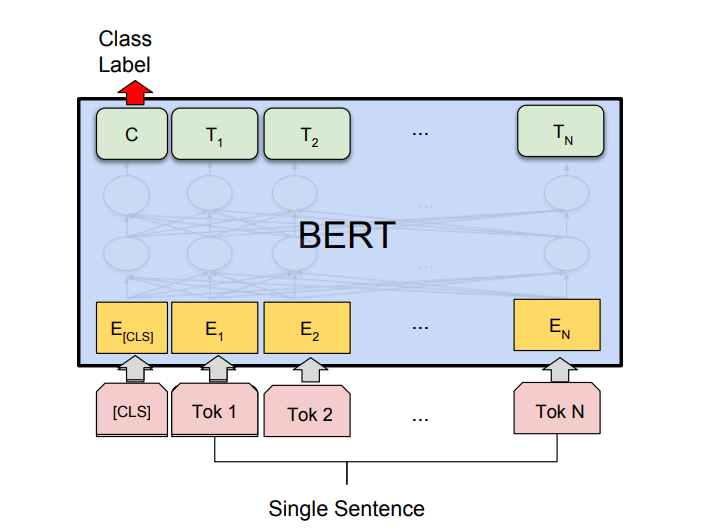
\includegraphics[width=0.5\textwidth]{pics/oth/bert for classification.png}
        \caption{Single sentence classification task, BERT}
        \label{fig:bert-classification}
    \end{figure}


    % leggere ulteriori informazioni dalle conclusioni del paper relativo a BERT (o introduzione o abstract o come vuoi insomma ciao)
    Tra i diversi impieghi del modello BERT è possibile usare il token specialce \textit{[CLS]} come illustrato in \ref{fig:bert-classification} per indicare il task di classificazione di una determinata frase. Dopo una prima fase di conversione delle parole in tokens il modello ne seleziona uno casualmente e, mascherandolo, cerca di predirlo autonomamente: questa procedura, chiamata dagli autori \textit{Masked LM}, forza la rete nel mantenere una rappresentazione del constesto distribuita su tutto il corpo della frase e non solo sui token antecedenti e successivi rispetto a quello considerato. La rappresentazione finale del testo, ottenuta leggendo gli output dell'ultimo layer del modello, permette una classificazione efficace in una delle classi che meglio descrive la frase fornita in input.

%!TEX root = ../thesis.tex
%*******************************************************************************
%****************************** Third Chapter **********************************
%*******************************************************************************

\chapter{Framework proposto}
\label{sec:FrameworkProposto}
\hspace{0,5cm}




\section{Overview del sistema proposto}

La ricerca svolta copre l'intero processo di raccolta e classificazione dei commenti partendo dalla raccolta dei dati fino al proponimento di diversi sistemi di riconoscimento dei discorsi d'odio. In figura \ref{fig:diag1} è proposto un diagramma di flusso descrittivo del percorso seguito durante lo studio. 

La prima fase fondamentale, utile a raccogliere il maggior numero di dati, è l'estrazione dei commenti da TikTok; successivamente le informazioni raccolte devono essere pulite dagli elementi poco utili ai fini della classificazione come messaggi di spam o eventuali errori.

Dopodiché vengono applicati e analizzati due metodi di classificazione differenti: il primo ha come obiettivo la segnalazione di lemmi offensivi o denigratori all'interno dei commenti, il secondo invece prevede il fine tuning di un modello per il riconoscimento del linguaggio naturale.


\begin{figure}[h!]
    \centering
    \includegraphics[width=0.7\textwidth]{pics/diagrams/flowchart thesis.png}
    \caption{Diagramma di flusso riepilogativo del lavoro svolto}
    \label{fig:diag1}
\end{figure}


Il primo metodo di classificazione prevede dapprima l'estrazione dei lemmi da ogni commento scaricato e, successivamente, un confronto con un lessico di termini offensivi e denigratori. Una volta ottenuti i risultati sarà possibile effettuare una valutazione qualitativa degli stessi per giudicare quanto il metodo di classificazione sia stato preciso nel riconoscere i commenti positivi da quelli offensivi.

Il secondo metodo di classificazione previsto dallo studio comprende l'utilizzo di un modello in grado di comprendere il linguaggio naturale sul quale effettuare fine tuning. Per questa fase è necessario classificare manualmente un sottoinsieme di commenti presi dai dati originariamente scaricati seguendo una serie di linee guida specificate in seguito. Come già visto per il metodo di classificazione precedente, viene effettuata una valutazione dei risultati in output adottando diverse configurazioni dei parametri della rete neurale profonda. Una volta trovata la migliore combinazione vengono svolte alcune ulteriori ottimizzazioni modificando la rete neurale per migliorarne ulteriormente le prestazioni. 

Tutti i risultati ottenuti vengono infine messi a confronto per determinare quale sia stato il miglior metodo di classificazione trovato.





\section{Raccolta e gestione dei dati}
In seguito alle restrizioni sulla privacy degli utenti nei social network nel corso degli ultimi anni, il processo di estrazione dati non può più essere svolto utilizzando delle API ufficiali. Nella maggior parte dei casi sono presenti tuttavia delle API non ufficiali che permettono di ottenere informazioni relative a singoli post o ad un singolo account. Nel caso specifico di TikTok, social network nato solo in tempi recenti, non sono presenti né API ufficiali né API alternative che permettono l'estrazione delle informazioni per la costruzione dei dataset utili alla ricerca. Per questo motivo è stato necessario costruire un tool in Python in grado di scaricare tutti i commenti da ogni post di un determinato account.

I dati raccolti vengono gestiti ed analizzati con l'ausilio di librerie quali Pandas e NumPy, universalmente utilizzati in presenza di grandi quantità di informazioni.

\subsection{Web scraping}
    Il Web scraping permette l'estrazione di dati da una pagina web simulando una navigazione di un normale utente. È stato utilizzato Selenium e Beautiful Soup rispettivamente per la simulazione della navigazione e la raccolta dei dati dalla struttura HTML della sezione commenti di ogni post. Si è reso altresì necessario adattare il più possibile il tool alle diverse configurazioni della pagina e ai vari sistemi di protezione che TikTok implementa per limitare la raccolta di dati automatica (Captcha in primis). Il processo per il download dei dati implica quindi l'apertura di un determinato post relativo ad un account, il caricamento di tutti i commenti e infine l'analisi dell'albero DOM (una rappresentazione a oggetti della pagina web) per l'estrazione del commento e dei suoi metadati. Per ogni commento vengono salvati il nome, l'identificativo univoco relativo all'account che ha commentato, l'immagine di profilo (utile per una successiva classificazione del genere) e il numero di like presenti al commento stesso.


\subsection{Pulizia dei dati}
    Prima dell'introduzione dei sistemi di identificazione dei discorsi d'odio ogni commento viene quanto più possibile pulito da ogni informazione accessoria non utile al processo di classificazione. Questa fase di pulizia dei dati è eseguita principalmente per minimizzare per quanto possibile la numerosità delle parole da analizzare e, di conseguenza, ottimizzare al meglio i tempi di calcolo richiesti nelle fasi successive.
    Per ogni commento vengono eliminati tutti i tag verso altri profili (e.g. \textit{@nomeprofilo}) e caratteri non standard che potrebbero creare problemi nella fase di analisi.
    Vengono anche riconosciuti ed eliminati manualmente messaggi di spam che riusultano poco utili nei vari passaggi di classificazione.





\section{Analisi del lessico}
Per una prima classificazione dei commenti scaricati viene utilizzato il lessico Hurtlex \cite{Hurtlex} contenente una raccolta di lemmi generalmente utilizzati nei commenti offensivi, aggressivi e denigratori. In particolare, ogni lemma appartiene ad una o più delle 17 categorie (quali ad esempio stereotipi etnici, disabilità fisiche, disabilità cognitive, omofobia, ecc.) e può essere classificato come conservativo o inclusivo. Nel primo caso il lemma ha un significato originale offensivo, nel secondo può assumere un significato offensivo solo se usato in determinati contesti. Si procede quindi con un confronto tra i lemmi che compongono i commenti scaricati e gli stessi riportati nel lessico, registrando la loro tipologia, la categoria di appartenenza e un identificativo univoco generato automaticamente.
    
\subsection{Lemmatizzazione}
    I dati originali vengono ulteriormente puliti prima di affrontare la fase di lemmatizzazione: punteggiatura, emoji, sequenze non appartenenti all'alfabeto e tutte le stop words, ovvero parole poco significative al senso finale della frase, non sono presenti nel lessico e pertanto sono inconcludenti ai fini della classificazione.
    Il risultato del precedente processo viene successivamente analizzato da Stanza \cite{Stanza}, una raccolta di modelli pre-addestrati dall'università di Stanford in grado di effettuare analisi sulla sintassi in varie lingue. 
    
    Per ogni parola di un commento viene estratto il lemma ottenendo la sua forma base e, successivamente, viene confrontato con con tutto il lessico Hurtlex. Tutti i commenti sono dunque classificati come non offensivi se nessun lemma ha trovato corrispondenza nel lessico o, come offensivi, se i commenti presentano uno o più lemmi segnalati nel lessico come potenzialmente denigratori.
    Per ciascun commento sono specificati gli id univoci dei lemmi potenzialmente offensivi e un punteggio basato sul numero di occorrenze per ogni categoria.






\section{Classificazione con BERT}
Una seconda possibilità di classificazione è data dall'utilizzo di reti neurali profonde in grado di riconoscere e interpretare il linguaggio naturale dei commenti. Viene utilizzata la tecnica del fine tuning che consente di usare una rete neurale già addestrata per un task generico e, ritoccandone i pesi, specializzarla per un task più specifico.

Data la complessità dei calcoli da svolgere e vista la dimensione della rete neurale profonda utilizzata, è stato necessario utilizzare hardware dedicato in grado di effettuare computazione parallela su schede grafiche Nvidia. Tra le diverse alternative si è scelta la piattaforma Colab di Google che permette la computazione in edge computing gratuitamente seppur con alcune limitazioni trascurabili sull'hardware e sui tempo di calcolo.

\subsection{Classificazione manuale e linee guida adottate}
    Durante il processo di fine tuning il modello necessita di dati etichettati da poter essere successivamente suddivisi in un dataset di train e un secondo dataset di test. È stato quindi necessario classificare manualmente un sottoinsieme di commenti originali in due classi: positivi e negativi. In questa fase delicata si è scelto di conservare quanto più possibile la tipologia di linguaggio e il gergo comune utilizzato su TikTok definendo delle linee guida da tenere a mente durante il processo di classificazione. 
    
    La classe di commenti positivi comprende non solo commenti generici ma anche quelli che mirano ad una difesa dell'influencer attaccato/a dai commenti classificati come negativi. Questa scelta rende sicuramente più difficile la fase di apprendimento visto l'utilizzo di un lessico molto simile tra commenti difensivi, classificati positivamente, e  quelli offensivi. Per descrivere al meglio la tipologia di classificazione appena esposta è di seguito fornito un esempio esplicativo a riguardo: "\textit{Wow mi hai migliorato la giornata}" e "\textit{Non ascoltare chi ti da della stupida}", sono entrambi classificati come commenti positivi mentre "\textit{Sei stupida e dovresti vergognarti}" è stato classificato come offensivo.
    
    La numerosità dei commenti negativi è risultata essere inferiore a quella dei commenti positivi a causa della moderazione effettuata già dal social network stesso al momento della pubblicazione. In totale sono stati classificati più di 2300 commenti di cui, circa il 15\% sono offensivi.

\subsection{Scelta del modello e fine tuning}
    La scelta del modello è sicuramente vincolata dalla lingua utilizzata nei commenti. Tra i diversi modelli a disposizione sulla piattaforma Huggingface \cite{huggingface} ne sono stati selezionati due per la lingua italiana: \textit{BERT base italian uncased} e \textit{BERT base italian xxl cased}: entrambi sono stati precedentemente addestrati dai laboratori di ricerca Google sul testo integrale di Wikipedia e su un corpus composto da articoli e testi ottenuti da pubblicazioni online. La principale differenza tra i due riguarda la dimensione del dataset utilizzato nella fase di addestramento iniziale e la capacità di saper riconoscere i caratteri maiuscoli da quelli maiuscoli. Sono stati considerati anche modelli capaci di riconoscere più lingue ma non verranno presi in considerazione nella fase sperimentale vista la loro bassa performance per la sola lingua italiana.
    
    
\subsection{Costruzione della rete neurale con BERT}
    Per poter controllare al meglio ogni parametro della rete neurale è stata scelta la libreria PyTorch \cite{pytorch}, ampiamente utilizzata nel mondo della ricerca per applicazioni riguardanti la visione digitale e l'elaborazione del linguaggio naturale.
    
    Dopo aver diviso il dataset prodotto dalla precedente fase di classificazione manuale ogni commento viene scomposto in tokens interpretabili dal primo layer di input del modello BERT. Più precisamente viene stimata una lunghezza massima fissata di 128 caratteri per commento anche se, mediamente, la lunghezza è di molto inferiore. Una volta generati gli input, ed effettuate le dovute conversioni in tensori, viene costruita una rete neurale semplice in grado di interpretare l'output del modello BERT selezionato precedentemente. La scelta dei parametri prende spunto dai consigli forniti dagli autori del modello stesso, sono state tuttavia apportate delle leggere modifiche al numero di epoche previste e alla dimensione di batch per cercare la combinazione che portasse al risultato migliore.
    
\subsection{Ottimizzazioni effettuate sulla rete neurale}
    Ottenuti i risultati dai due modelli BERT citati precedentemente si è scelto di ottimizzare al meglio la rete neurale per cercare di aumentare il più possibile la capacità di classificazione dei commenti offensivi e non. Vengono quindi effettuate una serie di modifiche eliminando l'ultimo layer da BERT dedicato alla classificazione (chiamato \textit{pooler layer}) in modo da aumentare la rete neurale di base con dei layer aggiuntivi, la cui scelta è influenzata dalle caratteristiche peculiari di quest'ultimi.
    
    L'elaborazione del linguaggio naturale, prima dell'arrivo dei modelli basati su reti di tipo transformer, era affidata alle reti neurali ricorrenti in grado di "ricordare", seppur in forma parziale, le informazioni date come input. Cercando di sfruttare questa caratteristica viene quindi introdotto un layer aggiuntivo di tipo Bi-LSTM, acronimo di \textit{Bi-directional long short term memory}. Lo scopo è quello di ottenere una rappresentazione eseguita dal modello BERT della frase in input e sfruttare le caratteristiche di memoria di una rete neurale ricorrente. Come anticipato si è scelto di utilizzare un layer di tipo Bi-LSTM che, grazie alla sua bidirezionalità, permette di accedere in ogni istante alle informazioni precedenti e successive riuscendo quindi a conservare il lavoro svolto da BERT nella rappresentazione del testo in input contemporaneamente rafforzando i pesi delle parole adiacenti a quella considerata.
    
    Una seconda opzione per migliorare le prestazioni è data dall'aggiunta di un layer lineare in coda al modello BERT. Questa tecnica permette di specializzare la rete per un task ancora più specifico migliorando quindi la rappresentazione del testo già effettuata da BERT. In seguito ad alcuni test è stato necessario inserire anche un layer di regolarizzazione in grado mitigare il fenomeno di overfitting. Verranno riportati i risultati ottenuti con un livello aggiuntivo di Dropout in grado di eliminare alcuni nodi presi in maniera casuale con una probabilità fissata dello 0.2\%.


%!TEX root = ../thesis.tex
%*******************************************************************************
%****************************** Third Chapter **********************************
%*******************************************************************************

\chapter{Risultati sperimentali}
\hspace{0,5cm} 


\section{Classificazione con il lessico Hurtlex}
I primi risultati ottenuti sono relativi alla classificazione con il lessico Hurtlex. Il lessico, composto da quasi 7000 lemmi molti dei quali inclusivi, riesce solo in parte a classificare correttamente i commenti in base alla loro categoria di appartenenza. Vengono quindi svolte alcune operazioni in grado di mitigare, anche se solo parzialmente, questo problema.

\subsection{Distribuzione delle categorie ed esempi descrittivi}
    Come descritto precedentemente ogni lemma contenuto nel lessico appartiene a una o più categorie. Tra le 17 categorie quella che ha una frequenza maggiore è quella relativa a \textit{parole dispregiative} seguita da termini relativi alla categoria \textit{omosessualità}. Tutte le altre categorie mantengono una frequenza che si attesta sullo stesso livello.
    
    Osservando i commenti, nello specifico quelli che presentano più segnalazioni, è possibile notare come il lavoro svolto dalla classificazione con il lessico Hurtlex non sia molto efficace nel trovare commenti con un senso offensivo. Nella maggior parte dei casi è possibile trovare commenti che contengono parole considerate offensive dal lessico ma che nella realtà sono applicate ad un contesto totalmente diverso da quello atteso. I falsi positivi risultano quindi essere gran parte dell'output prodotto dalla classificazione con il lessico Hurtlex. 
    
    Di seguito vengono riportati degli esempi esplicativi su quanto affermato in precedenza:
    nel commento "\textit{Sono cretina perché ancora non ti seguivo PS ti adoro}" il lemma segnalato è \textit{cretina} mentre invece in "\textit{sei bravissima e adoro il tuo stile faccio hip hop anche io, vorrei un sacco averti come insegnante ahaha}" viene sengalato il lemma \textit{insegnante}; in entrambi i casi però i commenti risultano essere totalmente inoffensivi.


\subsection{Distinzione tra lemmi conservativi e inclusivi}
    
    Per cercare di arginare il problema relativo alla segnalazione di commenti inoffensivi si è provato ad eseguire l'algoritmo di classificazione sfruttando solamente i termini conservativi che, a differenza dei termini inclusivi, assumono nella maggior parte dei contesti significati prettamente offensivi. In questo caso il numero di commenti segnalati è più basso rispetto alla classificazione precedente come osservabile dal grafico in figura \ref{fig:comments_distribution_conservative_barplot}.
    
    \begin{figure}[h]
        \centering
        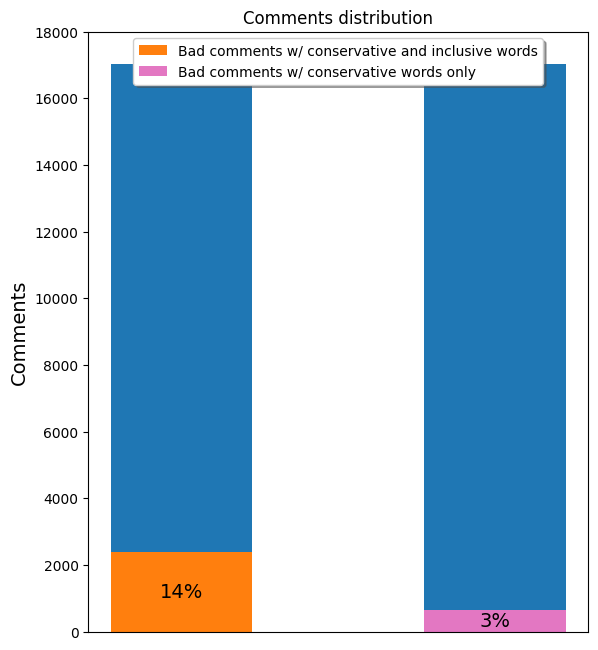
\includegraphics[width=0.5\textwidth]{pics/comments distribution conservative.png}
        \caption{Distribuzione dei commenti classificati come negativi usando lemmi conservativi e inclusivi o esclusivamente lemmi conservativi}
        \label{fig:comments_distribution_conservative_barplot}
    \end{figure}
    
    Nonostante l'utilizzo di lemmi solamente conservativi, la classificazione con il lessico non risulta comunque in grado di separare efficacemente i commenti offensivi da quelli innocui. I commenti segnalati quindi sono del tutto simili a quelli visti negli esempi precedenti. \\
    Dopo una veloce ispezione visiva dei commenti in output è possibile notare come, nonostante vengano selezionati commenti con parole offensive, spesso il contesto cambia il senso della frase. In altri casi invece i lemmi classificati come conservativi non hanno molto a che fare con contesti di offesa come è evidente da alcuni esempi che seguono: "\textit{Io sono due persone diverse praticamente}" e "\textit{Ma adesso che sono chiuse le discoteche come fai a lavorare? (Sembra una domanda aggressiva, ma sono solo curiosa)}" sono stati segnalati per la presenza del lemma \textit{diverso} nel primo commento e \textit{curioso} nel secondo.\\
    Inoltre è importante indicare come i commenti di difesa verso il/la creator di contenuti su TikTok vengano comunque segnalati come offensivi: nel commento "\textit{Ma che cafoni ignoranti! Sei bellissima!}" la presenza dei lemmi \textit{cafone} e \textit{ignorante} classifica automaticamente lo stesso come potenzialmente denigratorio.
    
    In generale, tra tutti i commenti segnalati, sono sicuramente presenti dei commenti offensivi ma, nonostante questo, il numero di falsi positivi rende la classificazione con il lessico Hurtlex poco efficace nell'isolare solamente i commenti negativi.
    




\section{Analisi esplorativa dei dati}
Una volta ottenuto un semplice metodo di classificazione dei commenti è possibile esplorare superficialmente le informazioni raccolte per riassumerne le principali caratteristiche. La numerosità del dataset complessivo supera i 250 000 elementi e, per ognuno, sono state registrate non solo le informazioni relative al corpo del commento ma anche i relativi metadati come le informazioni di base sul profilo proprietario e la data di pubblicazione dello stesso. Di seguito vengono quindi analizzati questi aspetti utili ad avere un quadro più chiaro sui dati a disposizione.

\subsection{Analisi di genere e movimenti temporali}
    
    Una prima considerazione viene svolta sulla distribuzione di genere di chi commenta. TikTok purtroppo non rende pubbliche le informazioni relative all'identificazione di genere di un account ed è stato quindi necessario classificare manualmente un campione di circa 10 000 account presi casualmente in base alla loro immagine profilo e ai contenuti caricati sulla piattaforma. La distribuzione risultante dall'analisi è osservabile nel grafico in figura \ref{fig:gendere distribution} dove è evidente come la presenza femminile sia di molto superiore rispetto alla controparte maschile.
    
    \begin{figure}[h]
        \centering
        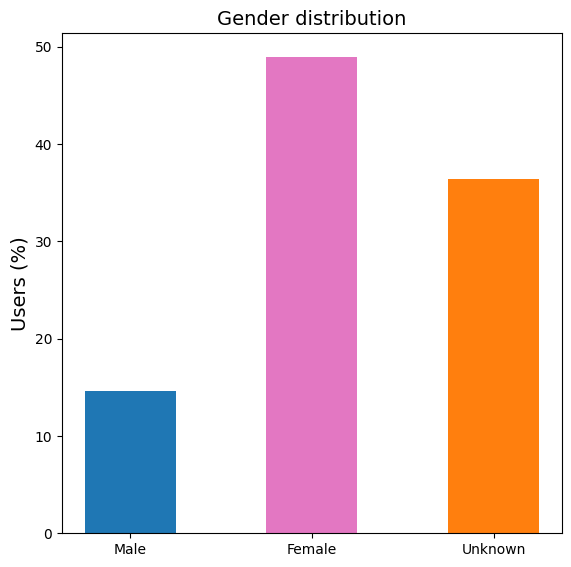
\includegraphics[width=0.5\textwidth]{pics/gender-distribution.png}
        \caption{Distribuzione di genere di un campione di 10 000 account}
        \label{fig:gendere distribution}
    \end{figure}
    
    
    Viene ulteriormente considerata la quantità di commenti segnalati durante il corso del tempo. Dopo aver collegato ogni commento al relativo post di appartenenza e conseguentemente diviso i dati in 10 regioni temporali, è stato possibile notare come la presenza di commenti negativi per ogni account si concentri sopratutto in presenza di post controversi che, diventando virali, attirano nuovi utenti che commentano negativamente. I picchi relativi a questo fenomeno sono osservabili nella figura \ref{fig:bins_total} suddivisi per i quattro account più popolari analizzati.
    
    \begin{figure}[h]
        \centering
        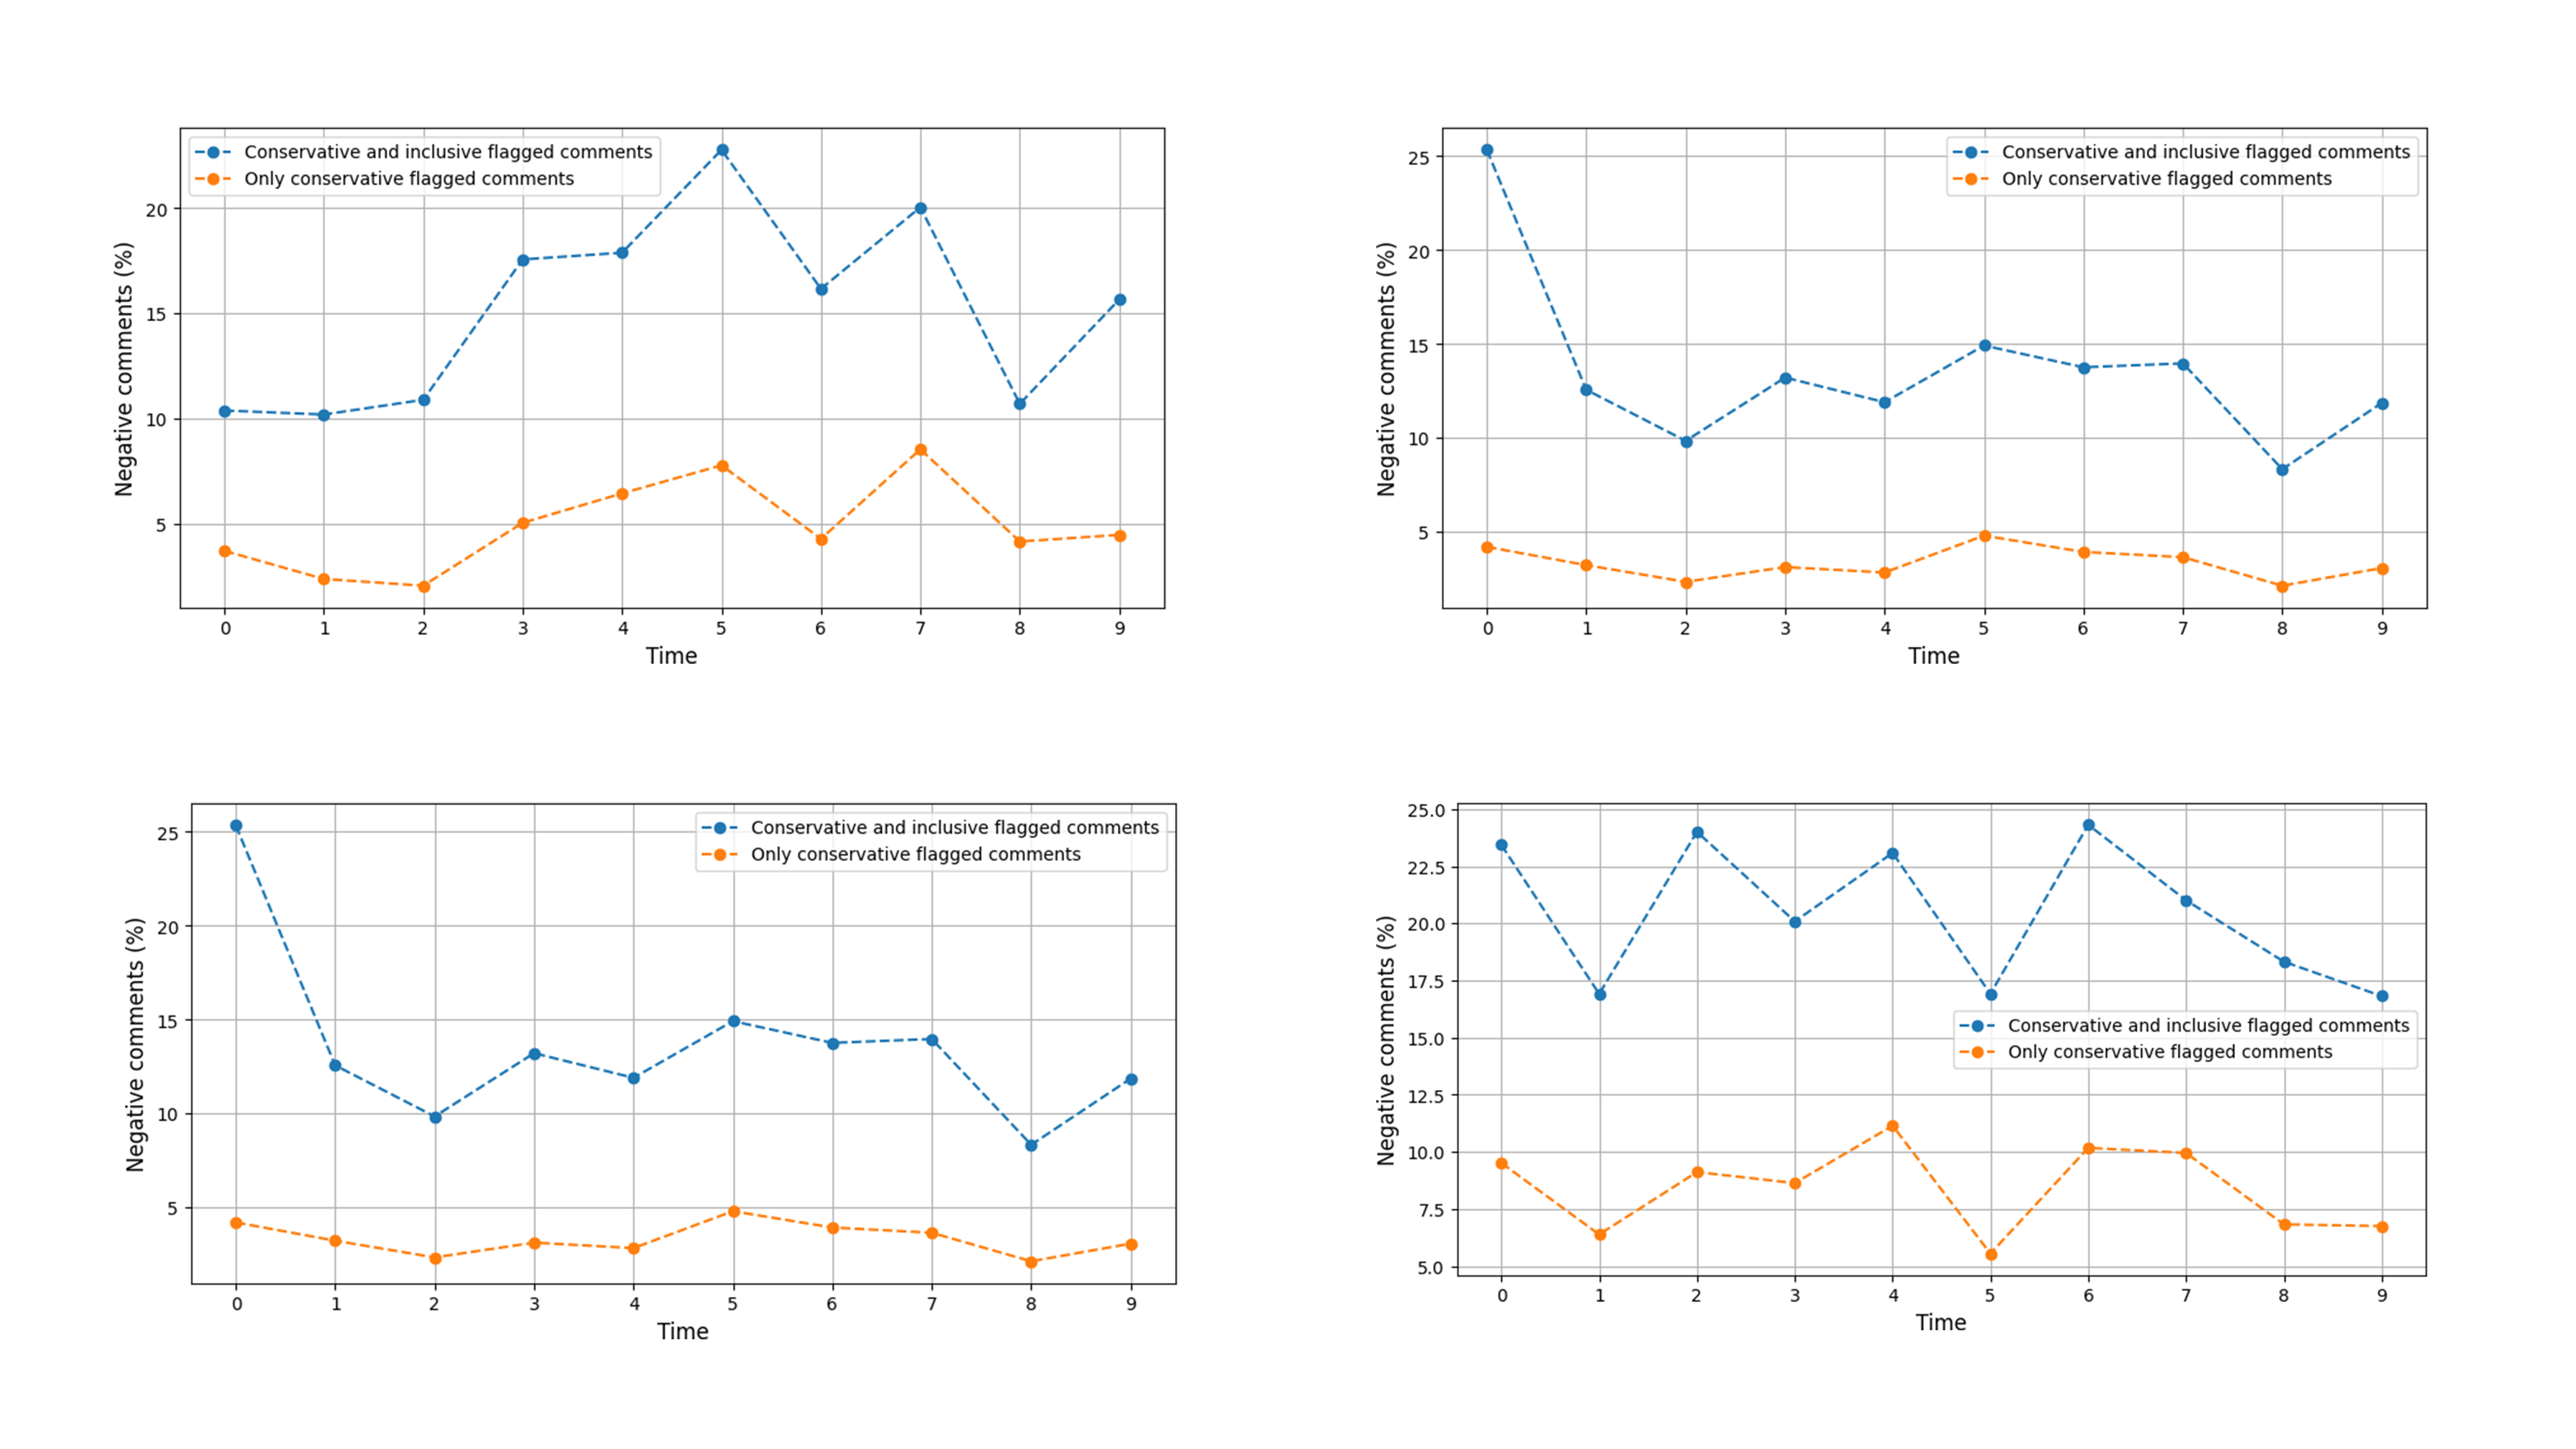
\includegraphics[width=1\textwidth]{pics/bins_comment-total.png}
        \caption{Movimenti temporali dei quattro account più popolari analizzati}
        \label{fig:bins_total}
    \end{figure}





\section{Fine tuning del modello BERT base}
Vengono proposti di seguito i risultati ottenuti dal processo di fine tuning dei modelli BERT descritti nel capitolo relativo al framework proposto. Per misurare la performance dei modelli e delle ottimizzazioni effettuate durante la fase di addestramento viene considerato l'output della funzione \textit{cross-entropia}, una funzione obiettivo (\textit{loss function}) che permette di avere una rappresentazione efficace sullo stato di apprendimento del modello. In seguito, per ogni epoca di addestramento effettuata, vengono considerate metriche quali F1, precisione e recupero osservando le rispettive matrici di confusione. L'accuratezza dei modelli non viene considerata ai fini della descrizione delle performance visto l'impiego di un dataset sbilanciato per la fase di addestramento e di test.


\subsection{Valutazione della funzione obiettivo}
    La valutazione della funzione obiettivo durante la fase di addestramento è essenziale per comprendere come il modello sta apprendendo le informazioni dai dataset di train e di test. Osservando i dati in output è possibile stabilire se la rete neurale si adatta eccessivamente ai dati di train. Questo fenomeno è definito come overfitting e può portare a basse performance per il dataset di test mantenendo allo stesso tempo delle ottime performance nel dataset di addestramento.
    
    La prima fase di test è stata effettuata variando lievemente i parametri consigliati dagli autori dei modelli basati su BERT per cercare quale configurazione di adattasse al meglio al task di classificazione considerato. Il training consiste in otto epoche totali dove, per ogni epoca, viene registrato l'output della loss function sia sul dataset di train che su quello di test. Viene inoltre considerata anche la lunghezza di un singolo batch facendola variare tra 16, 32 e 64. I risultati del primo modello \textit{BERT base italian uncased} vengono mostrati in figura \ref{fig:losses-uncased}.
    
    \begin{figure}[h]
        \centering
        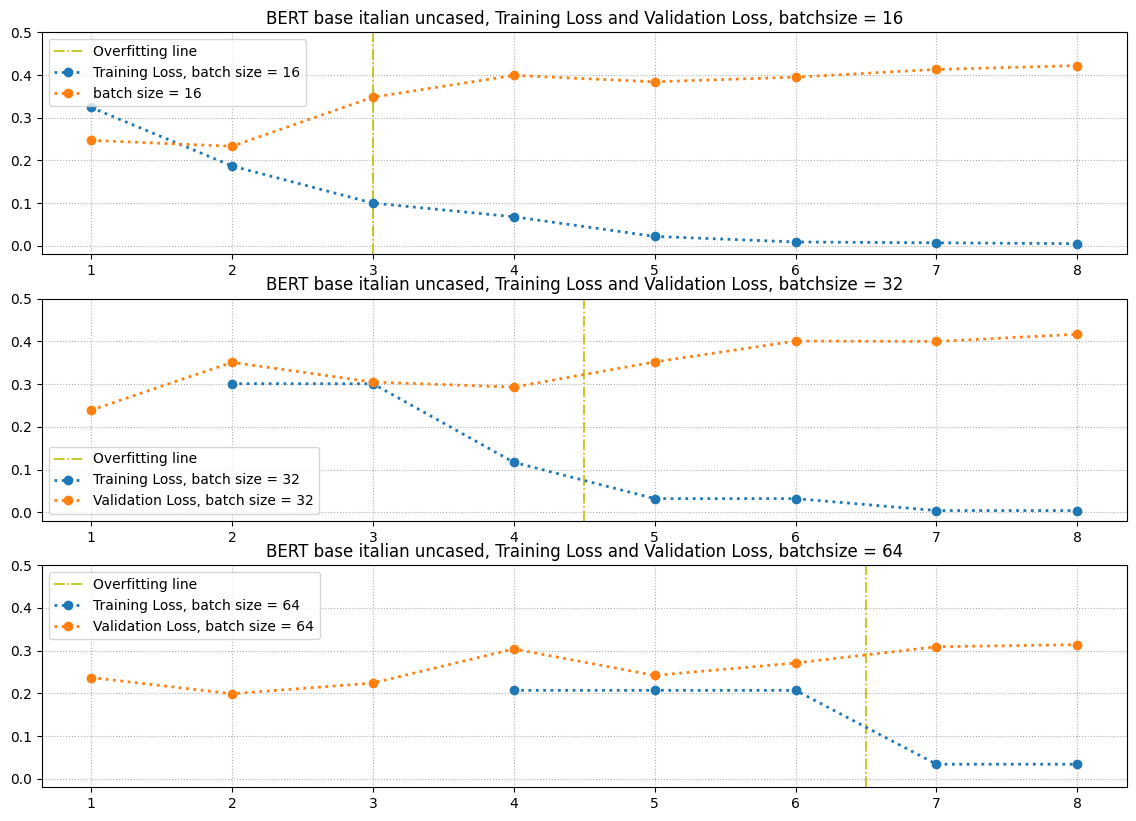
\includegraphics[width=0.65\textwidth]{pics/bert base italian uncased/losses.png}
        \caption{BERT base italian uncased; risultati funzione obiettivo per il dataset di train e di test}
        \label{fig:losses-uncased}
    \end{figure}
    
    
    I grafici ottenuti sono suddivisi secondo la lunghezza del batch utilizzata nella fase di addestramento. Come si può notare, osservando la crescita della funzione obiettivo per il dataset di test e la decrescita della stessa per il dataset di train, la probabilità di overfitting aumenta considerevolmente con l'aumentare delle epoche. Viene quindi rappresentata, attraverso l'utilizzo di una linea gialla, il limite entro il quale è consigliabile rimanere per il numero di epoche di addestramento necessarie al modello prima di incorrere in problemi di overfitting. I parametri ottimi ottenuti coincidono perfettamente con quelli consigliati dagli autori che suggeriscono un numero di epoche comprese nell'intorno di 4.
    
    
    \hspace{0,5cm}
    
    Il secondo modello utilizzato è \textit{BERT base italian xxl cased}. A differenza del modello visto precedentemente viene utilizzato un corpus maggiore nella fase di pre-training (un incremento di circa il 17\%) e viene aggiunta la capacità di riconoscere i caratteri minuscoli da quelli maiuscoli. L'output della funzione obiettivo è rappresentata in figura \ref{fig:losses-xxl}.
    
    \begin{figure}[h]
        \centering
        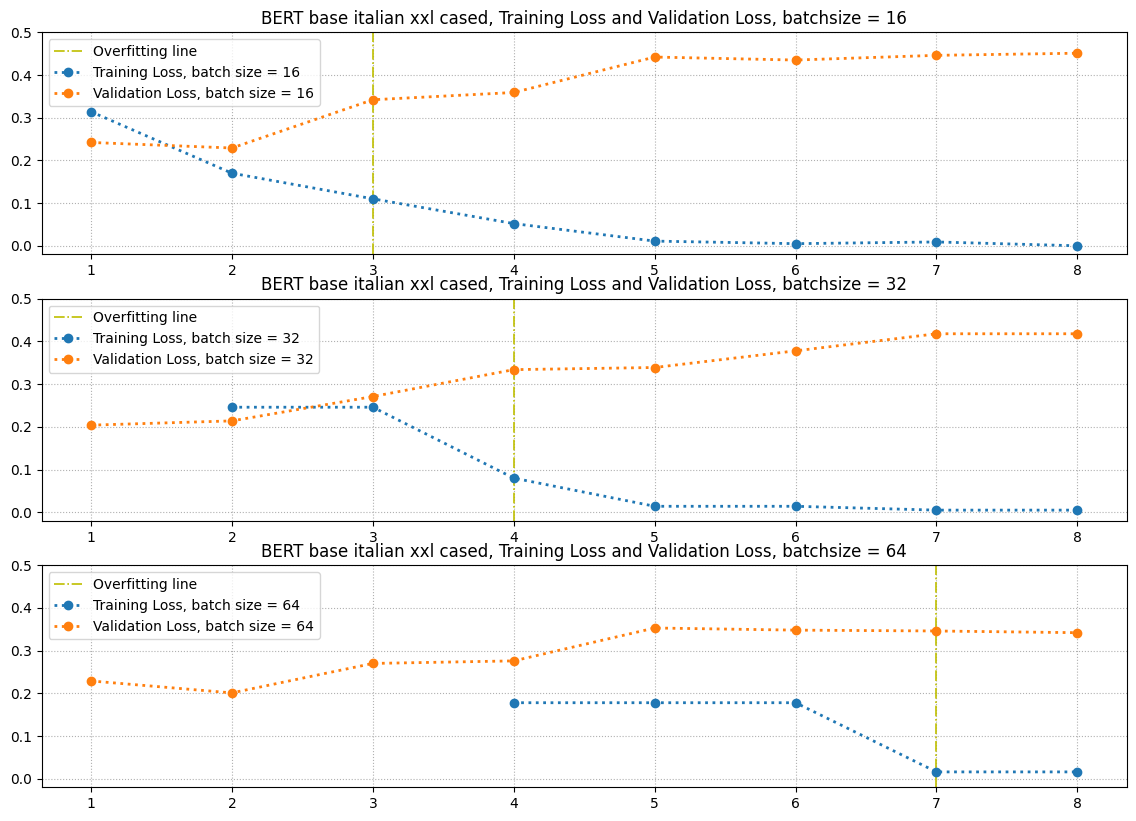
\includegraphics[width=0.65\textwidth]{pics/bert base italian xxl cased/losses xxl.png}
        \caption{BERT base italian xxl cased; risultati funzione obiettivo per il dataset di train e di test}
        \label{fig:losses-xxl}
    \end{figure}
    
    In entrambi i casi i risultati ottenuti riguardo il processo di apprendimento risultano essere molto simili. A seguito di ulteriori prove, aumentando fino a venti il numero di epoche, è possibile generalizzare l'andamento osservato: la probabilità di overfitting si presenta dopo un numero sempre maggiore di epoche proporzionalmente alla dimensione di batch.

\subsection{Metriche sul dataset di test}
    La valutazione del modello, come accennato precedentemente, è stata effettuata sul dataset di test dove ogni commento presente non è mai stato utilizzato per l'apprendimento nelle fasi precedenti. La scelta delle metriche è condizionata da alcuni fattori fondamentali dovuti alla distribuzione delle diverse classi nel dataset stesso. Nello specifico, avendo a disposizione un dataset sbilanciato, non è possibile usare l'accuratezza per descrivere al meglio il comportamento del modello nella fase di classificazione. Prendendo ad esempio il dataset a disposizione con solamente il 15\% di commenti negativi, il modello potrebbe classificare tutti i commenti come positivi e riuscire a raggiungere comunque un livello di accuratezza pari ad un 85\% senza in realtà classificare correttamente nessun commento negativo.
    
    La scelta della metrica ricade quindi sull'F1 score in grado di misurare l'accuratezza di un modello anche in caso di dataset sbilanciato. L'F1 score considera contemporaneamente sia la precisione che il recupero, due metriche utili a capire rispettivamente quanti commenti sono stati classificati correttamente sul totale dei commenti etichettati con una classe dal modello e quanti commenti sono stati correttamente classificati sul numero totale di commenti effettivamente appartenenti a quella classe. In termini più formali la precisione rappresenta il rapporto tra i veri positivi e la somma tra i veri positivi e i falsi positivi; il recupero è invece il rapporto tra i veri positivi e la somma dei vero positivi con i falsi negativi. Il punteggio F1 viene infine calcolato con la media armonica tra precisione e recupero definito di seguito:
    
    \[Precisione = \frac{VP}{VP + FP}\]
    
    \[Recupero = \frac{VP}{VP + FN}\]
    
    \[F_{1} = \frac{2}{\frac{1}{R} + \frac{1}{P}} = 2 \cdot \frac{P \cdot R}{P + R}\]
    
    Le metriche sopra descritte sono rappresentate in figura \ref{fig:f1-uncased} per il modello \textit{BERT base italian uncased} e in figura \ref{fig:f1-xxl} per il modello \textit{BERT base italian xxl cased}.

    \begin{figure}[h]
        \centering
        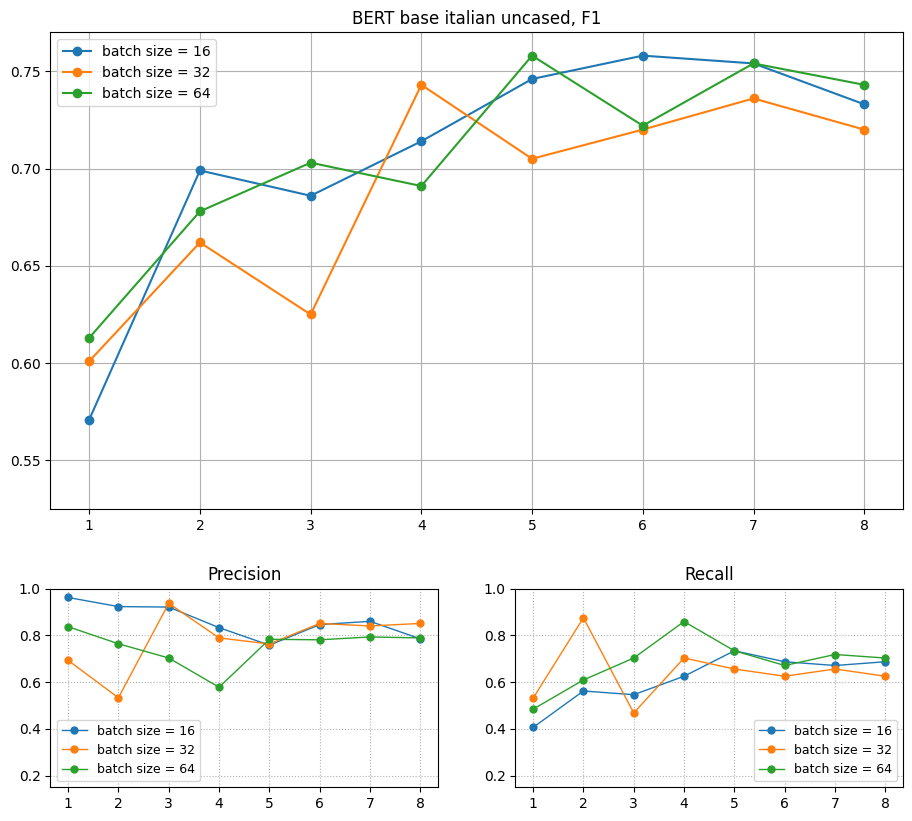
\includegraphics[width=0.8\textwidth]{pics/bert base italian uncased/f1 precision recall.png}
        \caption{\textit{BERT base italian uncased}; F1 score, precisione e recupero}
        \label{fig:f1-uncased}
    \end{figure}
    
    
    \begin{table}[h!]
        \centering
        \begin{tabular}{@{}lcccccc@{}}
        \toprule
                                  & \multicolumn{3}{c}{BERT base italian uncased} & \multicolumn{3}{c}{BERT base italian xxl cased} \\ 
        \multicolumn{1}{c}{Epoch} & 16 batch  & 32 batch   & 64 batch       & 16 batch          & 32 batch   & 64 batch     \\ \midrule
        1                         & 0.571     & 0.601      & 0.613          & 0.606             & 0.660      & 0.666        \\
        2                         & 0.699     & 0.662      & 0.678          & 0.756             & 0.736      & 0.716        \\
        3                         & 0.686     & 0.625      & 0.703          & 0.713             & 0.716      & 0.690        \\
        4                         & 0.714     & 0.743      & 0.691          & \textbf{0.760}    & 0.752      & 0.700        \\
        5                         & 0.746     & 0.705      & \textbf{0.758} & 0.735             & 0.737      & 0.699        \\
        6                         & 0.758     & 0.720      & 0.722          & 0.743             & 0.737      & 0.711        \\
        7                         & 0.754     & 0.736      & 0.754          & 0.735             & 0.728      & 0.733        \\
        8                         & 0.733     & 0.720      & 0.743          & 0.735             & 0.724      & 0.717        \\ \bottomrule
        \end{tabular}
        \caption{Risultati numerici per ogni epoca usando diverse dimensioni di batch}
        \label{Tab:f1-tab}
    \end{table}
    
    Confrontando i risultati ottenuti dai due modelli emerge una leggera superiorità per quanto riguarda il punteggio F1 ottenuto dal modello più grande \textit{BERT base italian xxl cased}. Osservando i valori numerici riportati in tabella \ref{Tab:f1-tab} sono evidenziati i punteggi F1 più alti ottenuti dai due modelli. Se si considera anche il numero di epoche, cercando di preferire il minor numero di iterazioni per evitare overfitting e abbassare i tempi di calcolo, il modello \textit{xxl} si conferma come il migliore tra i due considerati.
    
    \begin{figure}[h!]
        \centering
        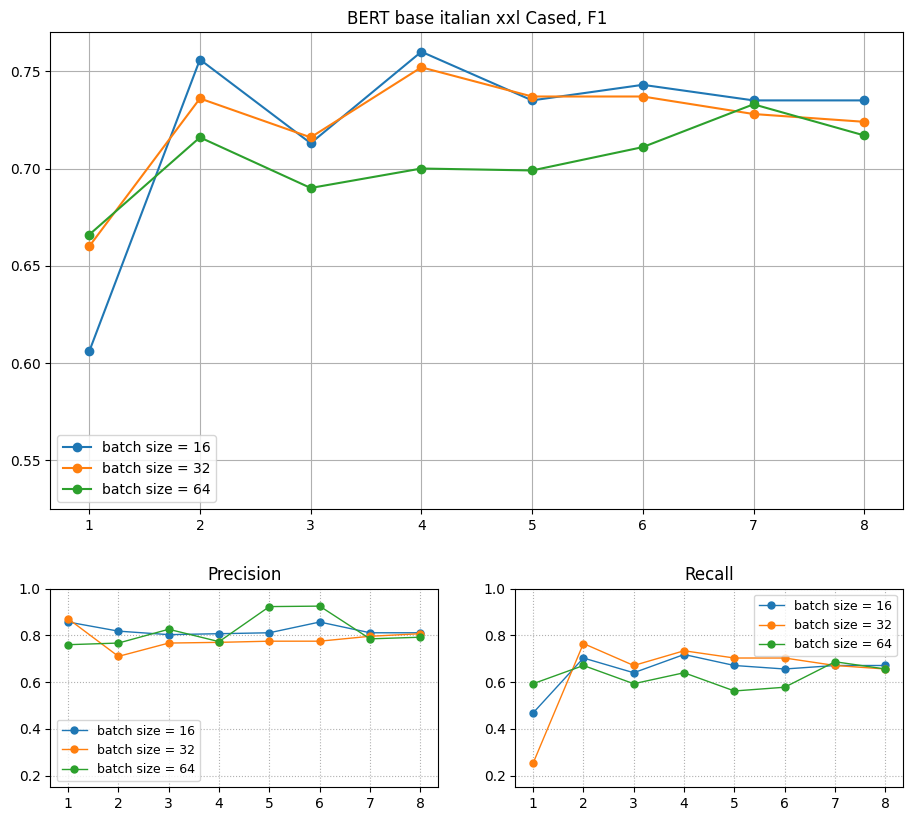
\includegraphics[width=0.8\textwidth]{pics/bert base italian xxl cased/f1 precision recall xxl.png}
        \caption{\textit{BERT base italian xxl cased}; F1 score, precisione e recupero}
        \label{fig:f1-xxl}
    \end{figure}
    
    La libreria PyTorch permette il salvataggio dei pesi trovati durante il processo di fine tuning del modello. Ricostruendo la rete neurale e importando i pesi precedentemente calcolati è possibile svolgere alcuni test manuali per osservare da più vicino il comportamento del modello nei diversi scenari di utilizzo. Le frasi più banali, la cui classe di appartenenza è ovvia anche con un semplice controllo del lessico, vengono classificate correttamente senza problemi mantenendo una probabilità restituita dalla funzione sigmoidea generalmente superiore al 85\%. Per mettere in difficoltà il modello è quindi necessario usare frasi che condividono lo stesso tipo di linguaggio ma con un significato diametralmente opposto. L'esempio riportato nella tabella \ref{Tab:class-example} mostra il risultato restituito dal modello in entrambi i casi. Nel secondo esempio è evidente come BERT non svolga solo un ruolo di classificazione basato sui termini utilizzati ma riesce efficacemente a comprendere il loro contesto di utilizzo interpretando correttamente il senso della frase. Viene ulteriormente segnalato come il problema dell'unintended bias nella classificazione dei discorsi d'odio (presentato e studiato in \cite{FersiniBias}) risulta essere efficacemente gestito dalla rete neurale testata.
    
    Rimane comunque importante sottolineare che la buona precisione riscontrata negli esempi riportati è dovuta alla forte presenza di termini simili nel dataset di train che permettono quindi un apprendimento efficace del modello stesso. Lo stesso comportamento non è sempre osservabile se si utilizzano vocaboli non presenti nel dataset di train dimostrando come, sopratutto quando si parla di reti neurali profonde, una grande quantità di dati risulta essere indispensabile per ottenere un modello che riesca a mantenere delle buone prestazioni anche nel mondo reale.
    
    \begin{table}[h]
        \centering
        \begin{tabular}{@{}lllc@{}}
        \toprule
          & \multicolumn{1}{l}{Commento} & Classe    & \multicolumn{1}{l}{Output funzione sigmoidea} \\ \hline %\cmidrule(l){1-4} 
        1 & \textit{Sei bravissima, complimenti}    & Good      &   0.06    \\
          & \textit{Sei bruttissimo, vergognati}    & Offensive &   0.97    \\
        \\
        2 & \textit{Dai, povero...}                  & Good      &   0.38    \\
          & \textit{Sei un povero}                  & Offensive &   0.78    \\ \bottomrule
        \end{tabular}
        \caption{Esempi di classificazione manuale per verificare la comprensione del contesto del modello BERT}
        \label{Tab:class-example}
    \end{table}
    
    
\section{Modifiche al modello BERT base}
I risultati ottenuti con l'utilizzo del modello base di BERT sono più che soddisfacenti per un semplice task di classificazione ma è possibile migliorare il risultato ottenuto aggiungendo dei layer che, invece di considerare l'output della classificazione (o pooler layer), raccolgono l'output dell'ultimo layer di BERT (768 nodi) e continuano il processo di fine-tuning.

Come accennato nel \hyperref[sec:FrameworkProposto]{capitolo relativo framework proposto} vengono proposte due modifiche diverse al modello BERT di base. La prima riguarda l'aggiunta di un layer di tipo Bi-LSTM in grado di memorizzare gli input antecedenti e seguenti, caratteristica peculiare delle reti neurali ricorrenti; la seconda riguarda l'aggiunta di un layer lineare, uno di dropout e infine un ultimo layer di output in grado di classificare nelle due classi gli input ricevuti. 

Come banchmark per il confronto delle prestazioni viene scelto il modello con i migliori risultati trovati nei capitoli precedenti: \textit{BERT base italian xxl cased} con una dimensione di batch pari a 16.

\subsection{BERT con layer Bi-LSTM}
    La prima modifica apportata al modello è stata aggiungere un layer Bi-LSTM in coda a BERT. Durante la fase di addestramento, osservando i risultati della funzione obiettivo per il dataset di train e di test in figura \ref{fig:bert-bi-lstm}, si può notare come i valori della loss function sul dataset di test aumentino dopo ogni epoca segnalando la probabile occorrenza di un problema di overfitting. Contemporaneamente la performance del modello, rappresentata dalla spezzata a destra, misurata dal punteggio F1 è in leggera discesa ma riesce a mantenere comunque dei valori in linea, o di poco inferiori, rispetto a quelli visti dal modello base di BERT.
    
    
    \begin{figure}[h]
        \centering
        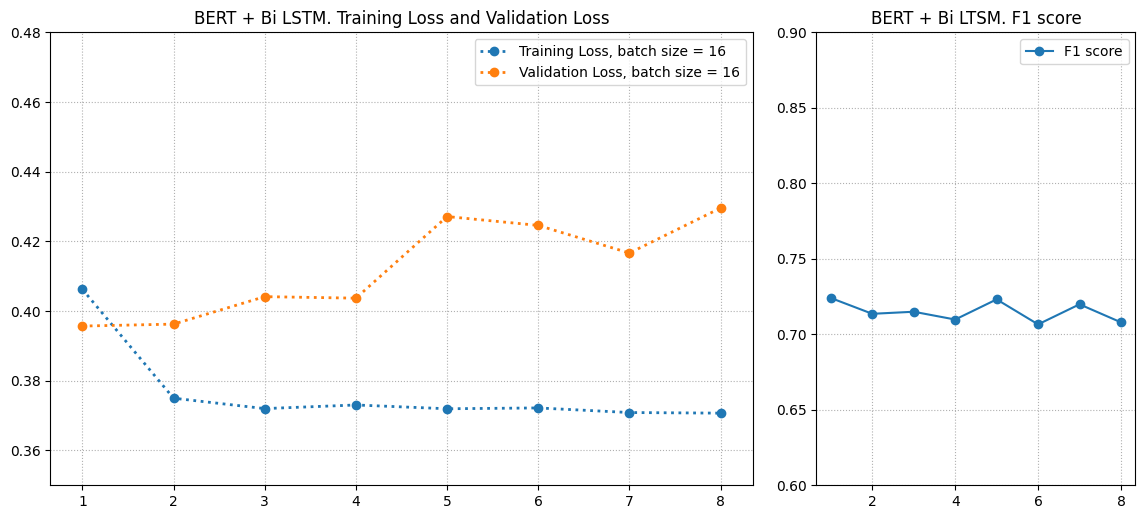
\includegraphics[width=0.8\textwidth]{pics/modifiche bert/BERT Bi LSTM.png}
        \caption{Metriche del modello BERT base con un layer Bi-LSTM in coda}
        \label{fig:bert-bi-lstm}
    \end{figure}
    
    
    A fronte di una validation loss maggiore e un punteggio F1 quasi identico al modello base di BERT è possibile concludere che questa modifica effettuata, almeno in questo caso, non porti a nessun vantaggio effettivo rispetto all'impiego del modello base. Questo comportamento è probabilmente attribuibile alla struttura delle reti neurali ricorrenti spiegate nel capitolo relativo al framework proposto. La loro capacità di ricordare è ristretta ai token vicini (destra e sinistra nel caso di una LSTM bidirezionale) e risulta essere quindi limitante rispetto all'ottima capacità di encoding di un'intera frase da parte delle reti neurali di tipo transformer di cui BERT fa parte.

\subsection{BERT con layer lineare, dropout e di classificazione}
    In figura \ref{fig:bert-linear} vengono rappresentati i risultati ottenuti dalla seconda modifica effettuata al modello base di BERT. In questo caso sono state effettuate diverse prove prima di ottenere il miglior risultato possibile. Inizialmente era stato utilizzato un singolo layer denso dimostratosi però inefficace nel migliorare le performance a causa del presentarsi di overfitting già dalla prima epoca. Si è quindi scelto di introdurre un layer di regolarizzazione, più nello specifico di dropout, per cercare di mitigare il problema di overfitting e subito dopo un semplice layer di classificazione in grado di restituire valori compatibili con le due classi dei commenti. Dopo diversi tentativi si è trovata la miglior percentuale di dropout fissata a 0.2. 
    
    \begin{figure}[h]
        \centering
        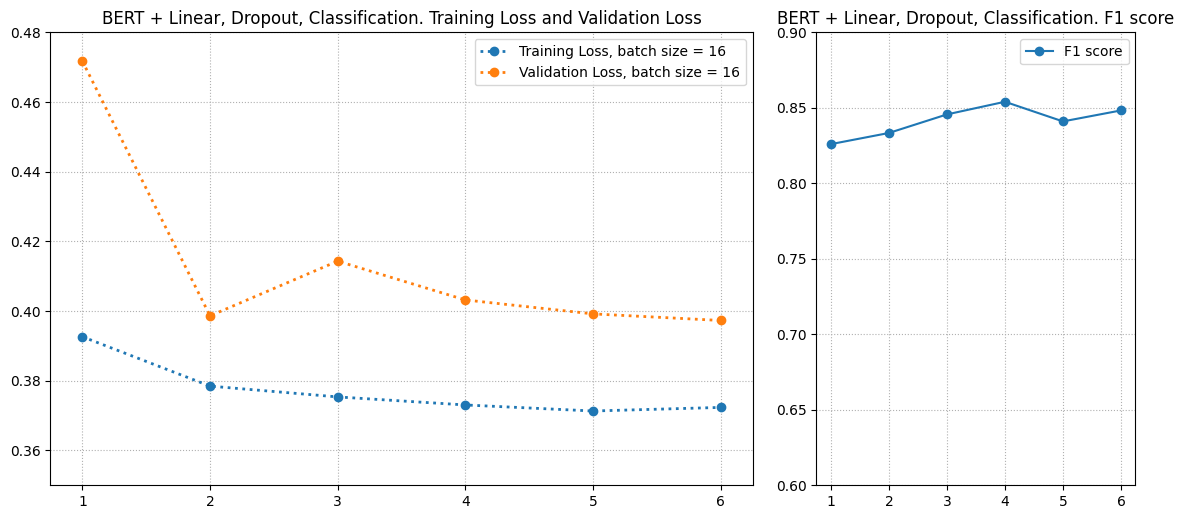
\includegraphics[width=0.8\textwidth]{pics/modifiche bert/BERT Linear.png}
        \caption{Metriche del modello BERT base con un layer lineare e uno di dropout in coda}
        \label{fig:bert-linear}
    \end{figure}
    
    I dati di classificazione ottenuti dimostrano come, nonostante una validation loss più alta della training loss in fase di training, le metriche sul dataset di test rimangano più che accettabili nel corso delle epoche. È possibile supporre che, in presenza di un dataset più grande nella fase di addestramento, i risultati della funzione obiettivo sarebbero stati sicuramente migliori: la rete neurale, con anche l'aggiunta dei nuovi layers visti precedentemente, risulta essere troppo grande per una quantità di dati così bassa.
    
\subsection{Confronto risultati con le modifiche effettuate}

    Viene infine proposto un grafico riassuntivo in figura \ref{fig:f1-comp-f} dove vengono illustrati i diversi punteggi F1 ottenuti sia dal modello base di BERT sia dai modelli con le modifiche apportate. Tra tutti i modelli proposti il migliore risulta essere BERT con i layer lineari e di dropout aggiunti in coda. Come anticipato il modello BERT base e il modello BERT con l'aggiunta di un layer Bi-LSTM si mantengono sulle stesse performance con un leggero vantaggio per il secondo a fronte però di una validation loss più alta vista precedentemente.
    
    
    \begin{figure}[h]
        \centering
        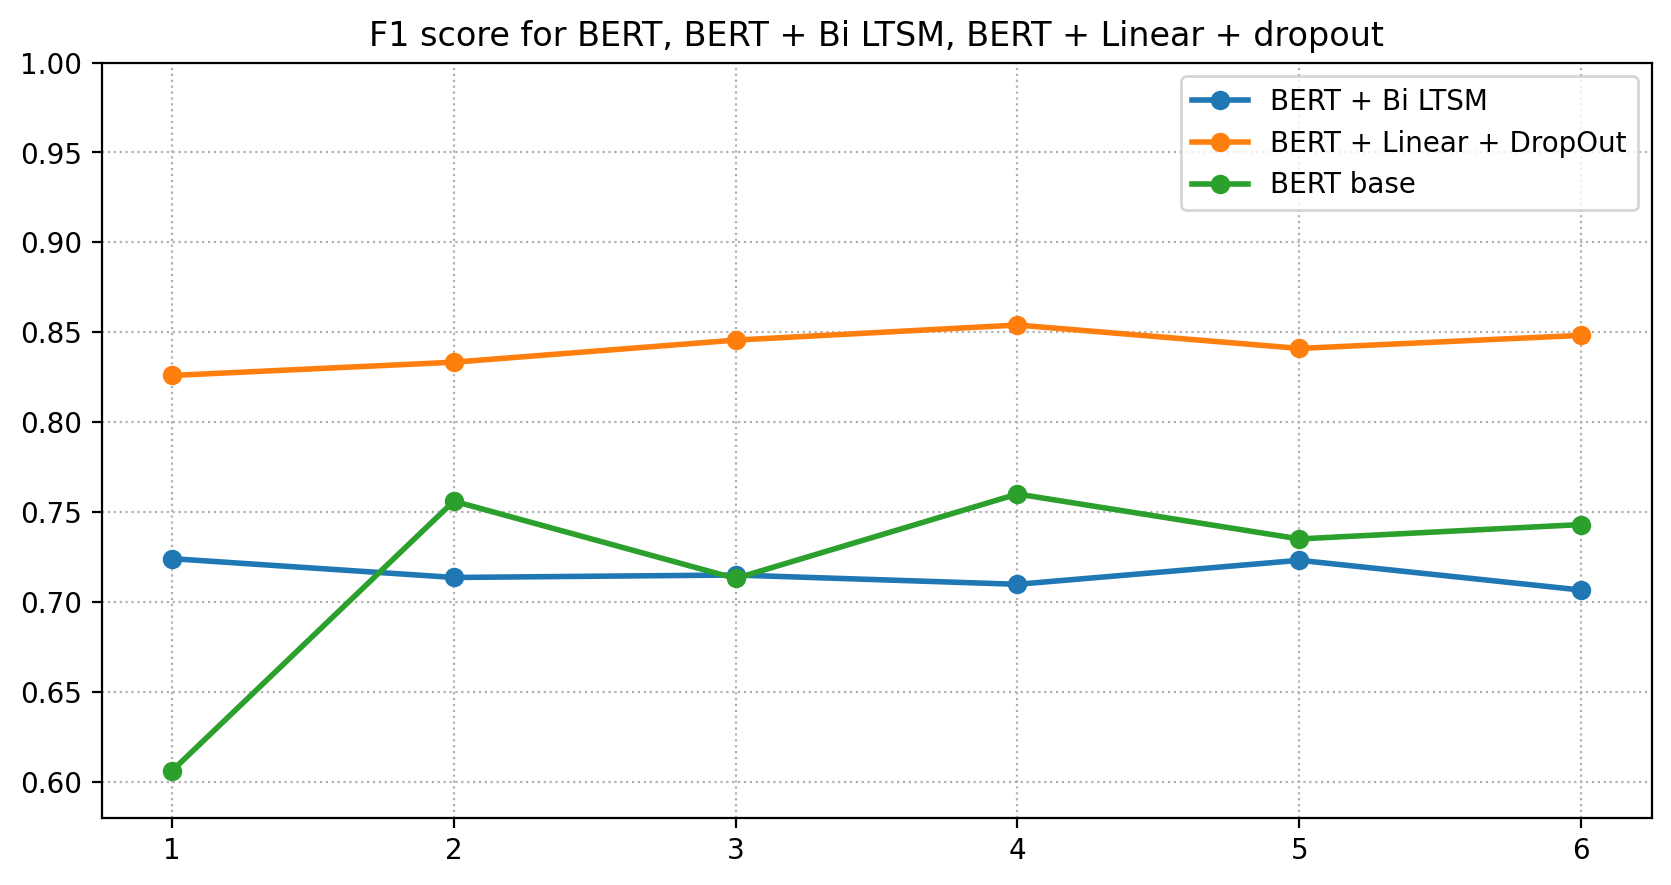
\includegraphics[width=0.8\textwidth]{pics/modifiche bert/F1 BERT Bi LSTM Linear stretched.png}
        \caption{Risultati ottenuti dal miglior modello BERT base e dai modelli modificati con i layer aggiuntivi}
        \label{fig:f1-comp-f}
    \end{figure}
    
    
    Nella tabella riepilogativa \ref{Tab:f1-comp-t} sono vengono ulteriormente riportati i punteggi F1 relativi alla prima classificazione con il lessico Hurtlex. Come previsto da una prima ispezione manuale, il lessico non è stato in grado di classificare efficacemente i commenti offensivi ottenendo un punteggio decisamente più basso dei modelli analizzati.
    
    \begin{table}[h]
    \begin{tabular}{@{}lcccccc@{}}
        \toprule
        Epoch & \begin{tabular}[c]{@{}c@{}}BERT\\ base\end{tabular} & \begin{tabular}[c]{@{}c@{}}BERT\\ Bi-LSTM\end{tabular} & \begin{tabular}[c]{@{}c@{}}BERT\\ Linear\\ dropout\end{tabular} & Hurtlex & \begin{tabular}[c]{@{}c@{}}Hurtlex\\ only\\ conservative\end{tabular}\\ \midrule
        %Epoch & BERT base & BERT + Bi-LSTM & BERT + Linear + dropout & Hurtlex   & Hurtlex only cons\\ \midrule
        1     & 0.606     & 0.724          & 0.825                   & -          & -           \\
        2     & 0.756     & 0.713          & 0.833                   & -          & -           \\
        3     & 0.713     & 0.714          & 0.845                   & -          & -           \\
        4     & 0.760     & 0.709          & \textbf{0.853}          & -          & -           \\
        5     & 0.735     & 0.723          & 0.840                   & -          & -           \\
        6     & 0.743     & 0.706          & 0.848                   & -          & -           \\ 
              & -         & -              & -                       & 0.121      & 0.154       \\\bottomrule
    \end{tabular}
    \caption{Tabella riepilogativa dei migliori risultati numerici ottenuti con tutti i metodi di classificazione utilizzati}
    \label{Tab:f1-comp-t}
    \end{table}
    
    
    
%!TEX root = ../thesis.tex
%*******************************************************************************
%****************************** Third Chapter **********************************
%*******************************************************************************
\chapter{Conlusioni e sviluppi futuri}
\hspace{0,5cm} 
\section{Conclusioni sul lavoro svolto}

La ricerca presenta una serie di valide proposte per la classificazione di commenti relativi ai discorsi d'odio online: i risultati ottenuti mostrano diverse strade percorribili ognuna con i propri vantaggi e svantaggi. È stato preso in analisi TikTok, un social network nato solo di recente, le cui dinamiche differiscono completamente da quelle tradizionali di piattaforme più conosciute e consolidate come Instagram, Twitter e Facebook. 


Dopo una prima fase di raccolta di dati, diversi sistemi di classificazione sono stati messi a confronto partendo dalla semplice analisi del lessico, fino ad arrivare all'uso di modelli rappresentanti lo stato dell'arte nel riconoscimento del linguaggio naturale.
Per la fase di addestramento della rete neurale è stato generato un dataset di commenti classificati manualmente definendo delle linee guida che permettessero al modello di apprendere la differenza tra un commento positivo e uno offensivo. È stata ulteriormente enfatizzata la differenza tra i commenti difensivi e offensivi che, pur condividendo gran parte del lessico, sono state distinte due classi diverse: questa scelta ha sicuramente influenzato le prestazioni del modello, il quale però ha dimostrato una buona capacità nel comprendere il contesto ivi una singola parola è inserita.

È stato successivamente applicato un processo di fine tuning che ha permesso la specializzazione della rete neurale in un task specifico riuscendo a migliorare di molto la precisione della classificazione. Una volta effettuati i diversi test ed aver trovato la combinazione di parametri migliori è stato altresì svolto un lavoro di ottimizzazione aggiungendo diversi tipi di layer dopo BERT che permettessero una maggiore specializzazione nel compito da svolgere. Tra le due prove effettuate solo la seconda, con l'aggiunta di layers lineari e di regolarizzazione, ha ottenuto prestazioni superiori, migliorando a tutti gli effetti la performance peraltro già molto buona di BERT. La prima prova invece, effettuata aggiungendo un layer di tipo Bi-LSTM, ha mantenuto delle performance quasi al pari di BERT per via dei suoi aspetti tecnici analizzati nei capitoli precedenti.


\section{Possibili miglioramenti proposti e sviluppi futuri}
È possibile estrapolare dal lavoro svolto alcuni possibili miglioramenti.

In primis, come accennato durante l'analisi dei risultati delle modifiche apportate a BERT, si è dimostrata necessaria l'analisi di un dataset dalle dimensioni maggiori. Le reti neurali profonde, come quelle utilizzate per la classificazione vista nei capitoli precedenti, necessitano di una grande quantità di dati per essere funzionali e mantenere le buone performance in un contesto reale, prescindendo da una classica fase di validazione.

Inoltre, con una maggiore quantità di dati, sarebbe possibile effettuare nuovi esperimenti partendo dalla base delle modifiche proposte o utilizzare nuovi modelli di base che migliorano le già ottime prestazioni di BERT (e.g. RoBERTa svilupatto dal Facebook AI in \cite{roberta}). Il problema principale, in entrambi i casi, è rappresentato dal fenomeno di overfittig che ha limitato la possibilità di ampliare ulteriormente la rete neurale o sfruttare appieno le caratteristiche intrinseche dei vari layer aggiunti.

Ultimo possibile miglioramento è rappresentato dal numero di features considerato dalla rete neurale. Nello studio riportato in tesi il modello riceve in input solamente il testo del commento, tuttavia viene ignorato il contesto entro il quale lo stesso è stato pubblicato. Di conseguenza in molti casi conoscere delle informazioni aggiuntive relative al post di provenienza o il commento principale in caso di una risposta a cascata, aiuterebbe nel compito di classificazione, fornendo ulteriori dettagli come base di partenza.






% ********************************** Back Matter *******************************
% Backmatter should be commented out, if you are using appendices after References
\backmatter

% ********************************** Bibliography ******************************
\begin{spacing}{0.9}

% To use the conventional natbib style referencing
% Bibliography style previews: http://nodonn.tipido.net/bibstyle.php
% Reference styles: http://sites.stat.psu.edu/~surajit/present/bib.htm

%\bibliographystyle{apalike}
%\bibliographystyle{unsrt}
 % Use for unsorted references  
%\bibliographystyle{plainnat} % use this to have URLs listed in References
\cleardoublepage
%\bibliographystyle{unsrt}
%\bibliography{References/references} % Path to your References.bib file
%\chapter*{Bibliografia}
ciao


% If you would like to use BibLaTeX for your references, pass `custombib' as
% an option in the document class. The location of 'reference.bib' should be
% specified in the preamble.tex file in the custombib section.
% Comment out the lines related to natbib above and uncomment the following line.

\printbibliography[heading=bibintoc, title={References}]


\end{spacing}

% ********************************** Appendices ********************************

 %\begin{appendices} % Using appendices environment for more functunality
%\appendixpage
%\include{Appendix/SubUniprot_text.tex}
%\appendix
%\chapter{Appendice}
%\input{Appendix/SubUniprot_text.tex}
%\input{Appendix/Textsubunit_analys.tex}
%\input{Appendix/dip_data.tex}
%\input{Appendix/subunit_find.tex}
%\input{Appendix/isoform_find.tex}
%\input{Appendix/CleanAndMerge.tex}
%\input{Appendix/CreateGPR.tex}
%\end{appendices}

% *************************************** Index ********************************
\markboth{}{}

% ringraziamenti qui dentro, if you like this
% \chapter*{Ringraziamenti}


\end{document}
